% Chapter generated from Part~II, Draft~10 by booktools/assemble.py
\begingroup
% macros of Part~II, Draft~10
\providecommand{\ov}{}\renewcommand{\ov}[1]{\overline{#1}}
\providecommand{\A}{}\renewcommand{\A}{\mathbb{A}}
\providecommand{\C}{}\renewcommand{\C}{\mathbb{C}}
\providecommand{\Z}{}\renewcommand{\Z}{\mathbb{Z}}
\providecommand{\cO}{}\renewcommand{\cO}{\mathcal{O}}
\providecommand{\fp}{}\renewcommand{\fp}{\mathfrak{p}}
\providecommand{\gen}{}\renewcommand{\gen}{\mathrm{gen}}
\providecommand{\reg}{}\renewcommand{\reg}{\mathrm{reg}}
\providecommand{\tr}{}\renewcommand{\tr}{\operatorname{tr}}
\providecommand{\Nrd}{}\renewcommand{\Nrd}{\operatorname{Nrd}}
\providecommand{\Ad}{}\renewcommand{\Ad}{\operatorname{Ad}}
\providecommand{\Iso}{}\renewcommand{\Iso}{\operatorname{Iso}}
\providecommand{\vol}{}\renewcommand{\vol}{\operatorname{vol}}
\providecommand{\supp}{}\renewcommand{\supp}{\operatorname{supp}}
\providecommand{\Cent}{}\renewcommand{\Cent}{\operatorname{Cent}}
\providecommand{\GL}{}\renewcommand{\GL}{\mathrm{GL}}
\providecommand{\St}{}\renewcommand{\St}{\mathrm{St}}
\providecommand{\Gb}{}\renewcommand{\Gb}{\ov{G}}
\providecommand{\Zb}{}\renewcommand{\Zb}{\ov{Z}}
\providecommand{\GDb}{}\renewcommand{\GDb}{\ov{G}_D}
\providecommand{\pib}{}\renewcommand{\pib}{\ov{\pi}}
\providecommand{\Eb}{}\renewcommand{\Eb}{\ov{E}}
\providecommand{\Tb}{}\renewcommand{\Tb}{\ov{T}}
\providecommand{\cG}{}\renewcommand{\cG}{\mathcal{G}}
\providecommand{\cGb}{}\renewcommand{\cGb}{\ov{\mathcal{G}}}
\providecommand{\iD}{}\renewcommand{\iD}{\iota_D}
\providecommand{\iG}{}\renewcommand{\iG}{\iota_{\GL}}
\providecommand{\jj}{}\renewcommand{\jj}{\jmath}
\providecommand{\sg}{}\renewcommand{\sg}{\sigma}
\providecommand{\Pv}{}\renewcommand{\Pv}{\textbf{(P)}}
\providecommand{\Ev}{}\renewcommand{\Ev}{\textbf{(E)}}
\providecommand{\Ov}{}\renewcommand{\Ov}{\textbf{(O)}}
\providecommand{\Cv}{}\renewcommand{\Cv}{\textbf{(C)}}
\chapter[Matching of arbitrary functions]{Matching of arbitrary functions and an improved global transfer}\label{ch:II}
\paragraph{Overview.} This is the second part of a study of a metaplectic Jacquet--Langlands transfer between the $n$-fold cover of $D^\times_{\A}$ constructed in \cite{JC26} and the Kazhdan--Patterson cover of $\GL(r,\A_K)$, where $D$ is a central division algebra of prime degree $r$ over a totally imaginary number field $K$ containing $\mu_n$, $n$ odd and $(n,r)=1$. Chapter~\ref{ch:I} proved matching of test functions supported on the regular set, and a transfer of packets under a non-cancellation hypothesis. Here we remove the regular-support condition. Near the center, an equivariant section of the cover, built from canonical $n$-th roots, identifies genuine functions on either cover with ordinary functions on the underlying linear group, with the same orbital integrals, compatibly with the identification of elliptic tori of Chapter~\ref{ch:I} (\emph{Theorem~D}). Combined with Chapter~\ref{ch:I} away from the center, this gives matching of arbitrary genuine test functions on the cover of $D_v^\times$, and of all genuine test functions with vanishing non-elliptic orbital integrals on the cover of $\GL(r,K_v)$ (\emph{Theorem~E}). Beyond the results imported from Chapter~\ref{ch:I} and the standard structure theory of the covers, the new external inputs concern the linear groups: orbital integrals of the Steinberg pseudo-coefficient and the linear transfer of cuspidal functions, which we derive from results of Flicker--Kazhdan and Badulescu. As an application we prove \emph{Theorem~C$'$}, an improvement of Theorem~C of Chapter~\ref{ch:I}: the packet identity holds with arbitrary matching test functions at all but one ramified place, and the non-cancellation hypothesis is replaced by a weaker one.

% =====================================================================
\section{Introduction}\label{II:sec:intro}
This section states the main results, explains how they improve the results of Chapter~\ref{ch:I}, fixes conventions and labels, and lists what is left after this chapter, with what Chapter~\ref{ch:III} has since done. It depends only on the statements of Chapter~\ref{ch:I}, and its notation is that of Chapter~\ref{ch:I}; all notation is collected in \S\ref{II:sec:glossary}, and the results are listed with their labels in the \hyperref[II:sec:summary]{Summary of results} that follows this section. References such as ``\cref{I:thm:easy}'' are to Draft~11 of Chapter~\ref{ch:I}, and \cite{JC26} refers to the corrected version of \cite{J88} (\texttt{metaplectic\_kazhdan\_revised12.tex}).

\subsection{Setting}
We use the global data of Chapter~\ref{ch:I} without change.

The standing assumptions are those of \cref{I:ass:standing}: $K$ is a totally imaginary number field containing $\mu_n$, with $n$ odd; $L/K$ is cyclic of prime degree $r$ with $(n,r)=1$; $D$ is a central division algebra over $K$ of dimension $r^2$ containing $L$; $S$ is the set of places where $D$ ramifies; and $c_v=r'c$ with $n\mid r-1+2rc_v$. Both the cover $\GDb(\A_K)$ of $D^\times_{\A}$ from \cite[\S6]{JC26} and the Kazhdan--Patterson cover $\Gb(\A_K)$ of $\GL(r,\A_K)$ with parameter $c_v$ are subgroups of one cover of $\GL(r,\A_L)$ (\S\S\ref{I:sec:covers} and \ref{I:sec:global}). We use the splitting conventions of \cref{I:lem:splittings}, good elements, the canonical identification $\jj$ of covered elliptic tori on good elements (\cref{I:thm:ident} and \cref{I:cor:classes}), the normalized orbital integrals $F=\Delta\Phi$ (\cref{I:def:oi}), and matching with the sign $(-1)^{r-1}$ (\cref{I:def:matching}).

\subsection{Main results}\label{II:subsec:main}
We state the three main results informally, with pointers to the precise statements.

Chapter~\ref{ch:I} left open the matching of test functions that do not vanish near the center: by \cref{I:prop:germ}, the orbital integrals of a genuine function $\tilde f_D$ on $\GDb(K_v)$ near the center are a nonzero constant times $\Delta$, so a matching function on $\Gb_v$ cannot be supported in the regular set. The key new tool is the following.

\begin{theoremD}[Propositions~\ref{II:prop:section} and~\ref{II:prop:transport}]
Let $v$ be a finite place. On a conjugation-invariant open and closed neighborhood $V$ of the unipotent set, the map $g\mapsto\sg(g):=\widetilde{g^{1/n}}^{\,n}$ (canonical $n$-th root, any lift, $n$-th power) is a well-defined continuous section of the cover. It is equivariant under conjugation, consists of good elements at regular points, agrees with the splittings over small open subgroups and over unipotent radicals, and is compatible with $\jj$. Genuine functions supported on $p^{-1}(ZV)$ correspond bijectively to ordinary functions on $G/Z$ supported on $ZV$, with the same orbital integrals, on both covers.
\end{theoremD}

Combined with Chapter~\ref{ch:I} away from the center, Theorem~D gives:

\begin{theoremE}[Theorem~\ref{II:thm:matching}]
Let $v\in S$. Every genuine test function on $\GDb(K_v)$ has a matching genuine test function on $\Gb_v$. Every genuine test function on $\Gb_v$ whose orbital integrals vanish at good regular non-elliptic elements has a matching function on $\GDb(K_v)$.
\end{theoremE}

The matching function in the first part of Theorem~E is explicit: $\tilde f=\tilde f_D(1)\,\tilde f^{\St}+\tilde f_{\reg}$, where $\tilde f^{\St}$ is the transport of the linear Steinberg pseudo-coefficient (\S\ref{II:subsec:steinberg}) and $\tilde f_{\reg}$ is supported on the good regular elliptic set. We also determine the germ near the center that any matching function must have (Theorem~\ref{II:thm:germ}).

Three objects should be kept apart: the Steinberg pseudo-coefficient $f_{\St}$ on $\GL(r,F)$; the genuine function $\tilde f^{\St}$ on $\Gb_v$, its transport near the center (cut off to a neighborhood of $\Zb_v$ and rescaled); and pseudo-coefficients of genuine irreducible representations of $\Gb_v$. The second is \emph{not} an instance of the third (Remark~\ref{II:rem:notpc}); matching needs only its orbital integrals.

\begin{theoremCp}[Theorems~\ref{II:thm:Cprime} and~\ref{II:thm:Cprimeconv}]
Let $\pib_D$ be a genuine automorphic representation of $\GDb(\A_K)$ with a supercuspidal component at a finite place $w_0\notin S$. The packet identity of Chapter~\ref{ch:I} holds with arbitrary matching test functions at all places of $S$ except one, $u$, which may be chosen freely. If the $D$-side packet satisfies the non-cancellation hypothesis $(\mathrm{Hyp}_D')$ (Definition~\ref{II:def:HDprime}), which is implied by the hypothesis $(\mathrm{Hyp}_D)$ of Chapter~\ref{ch:I}, then there is a genuine cuspidal automorphic representation $\pib$ of $\Gb(\A_K)$ with $\pib_v\cong\pib_{D,v}$ for all $v\notin S$. Conversely, if $\pib$ is the only member of its $\GL$-side packet and its components at the places of $S$ are square-integrable, then $\pib$ transfers to $\GDb(\A_K)$.
\end{theoremCp}

\subsection{What changes from Chapter~\ref{ch:I}}\label{II:subsec:changes}
We present every new global result as an improvement of a numbered result of Chapter~\ref{ch:I}. The following table is a guide for the reader of both chapters; each result in Chapter~\ref{ch:II} that improves a result of Chapter~\ref{ch:I} ends with a paragraph headed ``What changes from Chapter~\ref{ch:I}''.

\begin{center}
\begin{tabular}{>{\raggedright\arraybackslash}p{0.34\textwidth}>{\raggedright\arraybackslash}p{0.31\textwidth}>{\raggedright\arraybackslash}p{0.25\textwidth}}
\toprule
Chapter~\ref{ch:I} & Chapter~\ref{ch:II} & New input\\
\midrule
\cref{I:thm:easy} (Theorem~B: regular-supported matching) & Thm.~\ref{II:thm:matching} (Theorem~E: arbitrary functions) & Theorem~D; (L1), (L2)\\
\cref{I:prop:germ} (orbital integrals near $\Zb_v$, $D$ side) & Thm.~\ref{II:thm:germ} (required germ, $\GL$ side) & Theorem~D; measures\\
\cref{I:lem:Aprops} (regular support) & Lemma~\ref{II:lem:Aext} (arbitrary $\tilde f$) & Lemma~\ref{II:lem:singular}\\
\cref{I:def:globalpairs}, \cref{I:thm:comparison} (comparison) & Def.~\ref{II:def:uadm}, Thm.~\ref{II:thm:comparison2} & Theorem~E\\
\cref{I:prop:packet} (packet identity) & Prop.~\ref{II:prop:packet2} & Theorem~E\\
\cref{I:def:HD}, \cref{I:thm:transfer} (Theorem~C, $(\mathrm{Hyp}_D)$) & Def.~\ref{II:def:HDprime}, Thm.~\ref{II:thm:Cprime} (Theorem~C$'$, $(\mathrm{Hyp}_D')$) & Prop.~\ref{II:prop:packet2}\\
\cref{I:thm:converse}, \cref{I:rem:H} (converse, (Hyp)) & Thm.~\ref{II:thm:Cprimeconv}, Cor.~\ref{II:cor:Hprimesq} & Theorem~E(b); pseudo-coefficients\\
\cref{I:lem:cancel} (cancellation) & Prop.~\ref{II:prop:cancel2} & choice of $u$\\
\S\ref{I:sec:deferred}, items (D1)--(D4) & \S\ref{II:sec:partIII} & --\\
\bottomrule
\end{tabular}
\end{center}

\subsection{Logical structure}\label{II:subsec:deps}
The dependencies among the main results are as follows; arrows mean ``is used in''.
\begin{center}
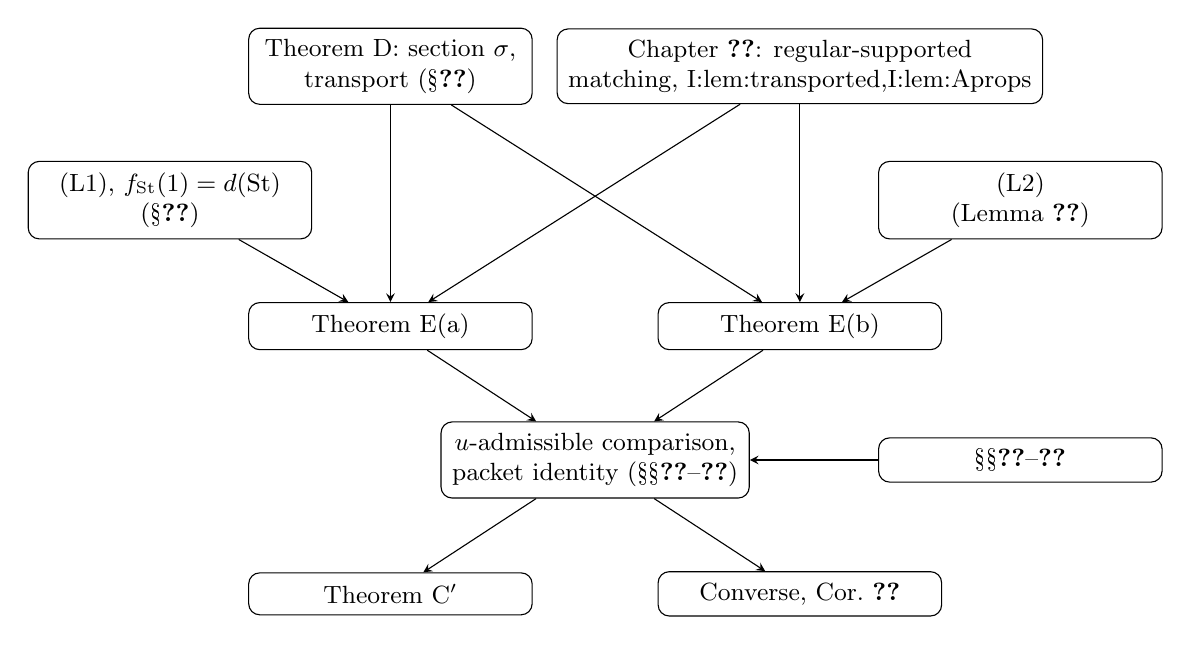
\begin{tikzpicture}[box/.style={draw,rounded corners,align=center,font=\small,inner sep=4pt,minimum width=3.6cm},>=stealth]
\node[box] (D) at (-2.6,0) {Theorem D: section $\sg$,\\ transport (\S\ref{II:sec:center})};
\node[box] (B) at (2.6,0) {Chapter~\ref{ch:I}: regular-supported\\ matching, \cref{I:lem:transported,I:lem:Aprops}};
\node[box] (L1) at (-5.4,-1.7) {(L1), $f_{\St}(1)=d(\St)$\\ (\S\ref{II:subsec:linear})};
\node[box] (L2) at (5.4,-1.7) {(L2)\\ (Lemma~\ref{II:lem:L2})};
\node[box] (Ea) at (-2.6,-3.3) {Theorem E(a)};
\node[box] (Eb) at (2.6,-3.3) {Theorem E(b)};
\node[box] (P) at (0,-5.0) {$u$-admissible comparison,\\ packet identity (\S\S\ref{II:subsec:uadm}--\ref{II:subsec:packet2})};
\node[box] (PI) at (5.4,-5.0) {\S\S\ref{I:sec:global}--\ref{I:sec:spectral}};
\node[box] (C) at (-2.6,-6.7) {Theorem C$'$};
\node[box] (Cc) at (2.6,-6.7) {Converse, Cor.~\ref{II:cor:Hprimesq}};
\draw[->] (D)--(Ea); \draw[->] (D)--(Eb); \draw[->] (B)--(Ea); \draw[->] (B)--(Eb);
\draw[->] (L1)--(Ea); \draw[->] (L2)--(Eb);
\draw[->] (Ea)--(P); \draw[->] (Eb)--(P); \draw[->] (PI)--(P); \draw[->] (P)--(C); \draw[->] (P)--(Cc);
\end{tikzpicture}
\end{center}
The germ results (Corollary~\ref{II:cor:germexp}, Lemma~\ref{II:lem:cuspnear1}, Corollary~\ref{II:cor:trivgerm}, Theorem~\ref{II:thm:germ}(b)) and the cancellation criterion (Proposition~\ref{II:prop:cancel2}) are not used in the proofs of Theorems~D, E and C$'$.

\subsection{Conventions and labels}\label{II:subsec:labels}
We keep the conventions and the labeling scheme of Chapter~\ref{ch:I}. They are collected, with the rest of the series' notation and the cocycle normalization, in the shared glossary of \S\ref{II:sec:glossary} (labels in \S\ref{gl:labels}, covers and the relabeling of $\mu_n$ in \S\ref{gl:cocycle}, Haar measures in \S\ref{gl:measures}).

All Hilbert symbols are $n$-th Hilbert symbols, and $\mu_n$ is relabeled once by $\zeta\mapsto\zeta^{r'}$ as in \S\ref{I:subsec:conventions}. Statements are marked by status, with proved-here the default and carrying no visible tag:

\emph{Proved here} (no tag): a complete argument is included, possibly using results marked \Ev. For global statements, ``proved'' means proved relative to the cited results of Chapter~\ref{ch:I}, which are restated in \S\ref{II:subsec:fromPartI}.
\begin{itemize}
\item \Ev\ \emph{Established elsewhere}: a precisely cited theorem, used as a black box. Several of these are results of Kazhdan \cite{Kaz86} that Flicker and Kazhdan state for covers in \cite{FK86}; we cite them in the form stated in \cite{FK86}.
\item \Ov\ \emph{Proof outlined}: the steps are identified, but at least one remains to be written out or checked.
\item \Cv\ \emph{Conjectural}: requires new mathematical input (later parts of the series).
\end{itemize}
A remark immediately after each \Ev, \Ov\ or \Cv\ statement explains its status.

\begin{center}
\begin{tabular}{>{\raggedright\arraybackslash}p{0.55\textwidth}>{\raggedright\arraybackslash}p{0.16\textwidth}>{\raggedright\arraybackslash}p{0.2\textwidth}}
\toprule
Statement & Where & Status\\
\midrule
Compatible measures at $S$; Chapter~\ref{ch:I} unaffected & \S\ref{II:subsec:measures} & \Pv\\
$n$-th roots; the section $\sg$; compatibility with $\jj$ (Theorem~D) & \S\S\ref{II:subsec:roots}--\ref{II:subsec:section} & \Pv\\
Transport; regular elements near $\Zb_v$ are good (Theorem~D) & \S\ref{II:subsec:transport} & \Pv\\
Germ expansion at central good elements & Cor.~\ref{II:cor:germexp} & \Pv\ using \Ev\\
Orbital integrals of arbitrary genuine functions ($r$ prime) & \S\ref{II:sec:arbitrary} & \Pv\\
Linear inputs (L1), (L2), $f_{\St}(1)=d(\St)$ & \S\ref{II:subsec:linear} & \Pv\ using \Ev\\
The pair $(e_D,\tilde f^{\St})$ & Prop.~\ref{II:prop:eD} & \Pv\\
Matching of arbitrary functions (Theorem~E) & Thm.~\ref{II:thm:matching} & \Pv\\
Required germ near the center: orbital-integral form & Thm.~\ref{II:thm:germ}(a) & \Pv\\
Unipotent orbital integrals of functions cuspidal near $1$; the trivial germ & Lemma~\ref{II:lem:cuspnear1}, Cor.~\ref{II:cor:trivgerm} & \Pv\ using \Ev\\
Required germ: unipotent form (G1), (G2) & Thm.~\ref{II:thm:germ}(b) & \Pv\\
Comparison and packet identity with $u$-admissible pairs & \S\S\ref{II:subsec:uadm}--\ref{II:subsec:packet2} & \Pv\ relative to Chapter~\ref{ch:I}\\
Theorem~C$'$ and its converse & \S\ref{II:subsec:Cprime} & \Pv\ relative to Chapter~\ref{ch:I}, under $(\mathrm{Hyp}_D')$, $(\mathrm{Hyp}')$\\
Cancellation criterion for $(\mathrm{Hyp}_D')$; finitely many $S$-types suffice & Prop.~\ref{II:prop:cancel2}, Cor.~\ref{II:cor:finiteStypes} & \Pv\\
Local character relations; unconditional transfer & \S\ref{II:sec:partIII} & \Cv\ (character relations at tame places: Chapter~\ref{ch:III})\\
\bottomrule
\end{tabular}
\end{center}

\subsection*{The running example}
The series' running example is $K=\mathbb{Q}(\zeta_3)$, $n=3$, $r=2$, $D=(-1,4-\zeta_3)_K$, ramified exactly at $S=\{\mathfrak p_3,\mathfrak p_7\}$, with $\mathfrak p_3=(1-\zeta_3)$ and $\mathfrak p_7=(3+\zeta_3)$ (Example~\ref{ex:running}, and \cite{JRE26}). Definition~\ref{II:def:measures} fixes $\mathrm{vol}(D_v^\times/F^\times)=d(\St)^{-1}$ at both places of $S$. Theorem~E applies at both. At the wild place $\mathfrak p_3$, where the covered elliptic tori are non-abelian, matching near the center uses Theorem~D. In Theorem~C$'$ the place $u$ is $\mathfrak p_3$ or $\mathfrak p_7$, and $(\mathrm{Hyp}_D')$ is a condition on test functions at these two places.

\subsection{Organization}
Section~\ref{II:sec:recall} recalls what we use from Chapter~\ref{ch:I} and fixes the Haar measures at the ramified places. Sections~\ref{II:sec:center}--\ref{II:sec:matching} contain the local theory: the section $\sg$ and the transport (\S\ref{II:sec:center}), orbital integrals of arbitrary genuine functions away from the center (\S\ref{II:sec:arbitrary}), and matching of arbitrary functions (\S\ref{II:sec:matching}). Section~\ref{II:sec:CC} proves Theorem~C$'$. Section~\ref{II:sec:partIII} lists what is left for Chapter~\ref{ch:III}. Section~\ref{II:sec:glossary} collects the notation of the series and the notation specific to Chapter~\ref{ch:II}, and Section~\ref{II:sec:lit} discusses the work related to this Part; the literature of the whole series is reviewed in \S\ref{I:sec:lit}.

% =====================================================================
\section{Recollections from Chapter~\ref{ch:I}, and Haar measures}\label{II:sec:recall}
This section recalls the notation of Chapter~\ref{ch:I} that is used throughout, and fixes the Haar measures at the ramified places once and for all. It depends only on Chapter~\ref{ch:I}, whose results used here are restated in \S\ref{II:subsec:fromPartI} as (I1)--(I11). It introduces the local notation $P_g$, $A_g$, $\Phi^z$, the compatible measures of Definition~\ref{II:def:measures}, and the constant $\lambda_v$.

\subsection{Local notation}\label{II:subsec:localnotation}
We fix the local notation used in \S\S\ref{II:sec:center}--\ref{II:sec:matching}.

Throughout \S\S\ref{II:sec:center}--\ref{II:sec:matching}, $v$ is a finite place, $F=K_v$, $\fp$ its maximal ideal, $\varpi$ a uniformizer and $p$ the residual characteristic. We write $G$ for either $\GL(r,F)$ (embedded in $\cG_v$ by $\iG$) or $D_v^\times$ (embedded by $\iD$), $\Gb=p^{-1}(G)\subset\cGb_v$, $Z=F^\times$ and $\Zb=p^{-1}(Z)$, which is central and common to both covers (\cref{I:lem:center}). For $g\in G$ let $P_g$ be its characteristic polynomial (reduced characteristic polynomial if $G=D_v^\times$), $A_g:=F[g]$ the commutative $F$-algebra it generates, and call the roots of $P_g$ in $\ov F$ the eigenvalues of $g$. For a genuine character $\tilde\theta$ of $\Zb$, $C_c^\infty(\Gb,\tilde\theta)_\gen$ is the space of smooth genuine functions with $\tilde f(z\tilde g)=\tilde\theta(z)^{-1}\tilde f(\tilde g)$ and support compact modulo $\Zb$. Orbital integrals $\Phi$ and $F=\Delta\Phi$ are those of \cref{I:def:oi}, with $\Delta(\gamma)=|D(\gamma)|^{1/2}|\det\gamma|^{-(r-1)/2}$; as in \cite[\S6]{FK86}, $D(\gamma)$ is formed from the distinct eigenvalues. We also use the variant $\Phi^z(\gamma,f)=\int_{Z\backslash G}f(g^{-1}\gamma g)\,dg$ of \cite[\S6]{FK86} for regular elliptic $\gamma$; then $\Phi^z(\gamma,f)=\vol(T_\gamma/Z)\,\Phi(\gamma,f)$.

\subsection{Haar measures at the ramified places}\label{II:subsec:measures}
We fix compatible Haar measures at the places of $S$ (Definition~\ref{II:def:measures}), used in the rest of the chapter. This choice is made once and for all; it simplifies the normalization at the identity and the formal-degree relations of \S\ref{II:sec:partIII}(ii).

Measures are as in \S\ref{I:subsec:oi}: $dg$ on $G/Z$, $dt$ on $T/Z$, and $dg/dt$ on $T\backslash G$; at $v\in S$ they are specialized as follows.

\begin{definition}[Compatible measures]\label{II:def:measures}\index{compatible measures@Compatible measures}
At each $v\in S$, let $dg_v$ be any Haar measure on $\GL(r,F)/F^\times$, and let $d(\St)=d(\St;dg_v)$ be the formal degree, with respect to $dg_v$, of the Steinberg representation of $\GL(r,F)$ (trivial central character). Normalize the Haar measure $dg_{D,v}$ on the compact group $D_v^\times/F^\times$ by
\[ \vol(D_v^\times/F^\times;\,dg_{D,v})=d(\St;dg_v)^{-1}. \]
The measures $dt$ on tori are arbitrary, as in Chapter~\ref{ch:I} (matching does not depend on them).
\end{definition}

\begin{remark}\label{II:rem:measures}
(1) \S\ref{I:subsec:measures} allows arbitrary $dg_v$ and $dg_{D,v}$ at $v\in S$, provided matching and the trace formulas use the same ones. So every result of Chapter~\ref{ch:I}, local and global, holds with the measures of Definition~\ref{II:def:measures}, and we cite Chapter~\ref{ch:I} without change.

(2) The formal degree of the trivial representation of $D_v^\times$ is $\vol(D_v^\times/F^\times)^{-1}$, and the trivial representation corresponds to $\St$ under the linear Jacquet--Langlands correspondence \cite[Theorem~2.2]{Bad08}. So Definition~\ref{II:def:measures} says that this pair has equal formal degrees. We expect that it agrees with Kottwitz's normalization of measures on inner forms \cite{Kot88}, but nothing below uses this.

(3) For arbitrary measures, the constant $\lambda_v:=d(\St)\vol(D_v^\times/F^\times)$ would appear in the normalization at the identity (Theorem~\ref{II:thm:germ}(c)). Definition~\ref{II:def:measures} is exactly the condition $\lambda_v=1$.
\end{remark}

\subsection{Statements used from Chapter~\ref{ch:I}}\label{II:subsec:fromPartI}
For the reader's convenience, and to make the dependence on Chapter~\ref{ch:I} auditable, we restate the results of Chapter~\ref{ch:I} that are used, in the form used. Numbers refer to Chapter~\ref{ch:I}. The labels (I1)--(I11) are used in the rest of the paper.

\begin{enumerate}[label=(I\arabic*)]
\item \emph{Admissible functions} (\S\ref{I:subsec:transported}). For $\bullet\in\{D,\GL\}$ and an elliptic torus of type $i$, a function $h$ on the good regular elements $Z(\Eb_{i,\bullet})^{\reg}$ is admissible if it is (i) locally constant, (ii) satisfies $h(z\tilde t)=\tilde\theta_v(z)^{-1}h(\tilde t)$ for $z\in\Zb_v$, (iii) has support compact modulo $\Zb_v$ with closure contained in the regular set, and (iv) is invariant under the normalizer of the torus.
\item \emph{\Cref{I:lem:transported}.} (b) $h\mapsto h\circ\jj_i^{-1}$ is a bijection between admissible functions on the two sides. (c) Every admissible $h$ equals $F(\cdot,\tilde f_i)$ on $Z(\Eb_{i,\bullet})^{\reg}$ for some $\tilde f_i\in C_c^\infty$ supported on the good regular elements conjugate into that torus; $F(\tilde\delta,\tilde f_i)=0$ for regular $\tilde\delta$ not conjugate into it.
\item \emph{\Cref{I:thm:easy}.} (a) Every $\tilde f_D$ vanishing near $\Zb_v$ has a matching $\tilde f$ supported on the good regular elliptic set. (b) Every $\tilde f$ supported in the regular set with vanishing orbital integrals at good regular non-elliptic elements has a matching $\tilde f_D$ vanishing near $\Zb_v$.
\item \emph{\Cref{I:prop:germ}.} For $\tilde f_D$ there are a normal open compact $U\subset D_v^\times$ and a splitting $\kappa_U$ with $F(z\kappa_U(t),\tilde f_D)=\Delta(t)\vol(T\backslash D_v^\times)\tilde f_D(z)$ for $z\in\Zb_v$ and regular $t\in U$.
\item \emph{\Cref{I:lem:Asub}(b)} (Harish-Chandra). For $C\subset T^{\reg}$ and $\Omega\subset G$ compact modulo $Z$, the set of $\dot x\in T\backslash G$ with $x^{-1}Cx\cap\Omega\ne\emptyset$ is compact. (Stated in Chapter~\ref{ch:I} for any such $\Omega$.)
\item \emph{\Cref{I:lem:Aprops}.} For regular-supported $\tilde f$, $F(\cdot,\tilde f)$ on an elliptic torus is admissible. \emph{\Cref{I:lem:traceOI}.} Traces of regular-supported functions depend only on their good regular orbital integrals.
\item \emph{\Cref{I:prop:geomD}.} The $D$-side trace formula: $\sum m(\pib_D)\tr\pib_D(\tilde f_D)=\vol\cdot\tilde f_D(1)+\sum_{[\gamma]}c(\gamma)F(\iota(\gamma),\tilde f_D)$, the sum over rational regular classes modulo the center that are good everywhere; every non-central rational element of $G_D(K)$ is regular since $r$ is prime. No condition on the test function at $S$.
\item \emph{\Cref{I:prop:FKvariant}} (variant of \cite[\S18]{FK86}). For $\tilde f$ with (i) a supercusp form at some finite place $w_0$ and (ii) support in the regular elliptic set at some finite place $u$, and no condition elsewhere: $\sum_{\text{cuspidal}}m(\pib)\tr\pib(\tilde f)=\sum_{[\gamma]}c(\gamma)F(\iota(\gamma),\tilde f)$, the sum over rational regular elliptic classes good everywhere.
\item \emph{\Cref{I:thm:rational} and \cref{I:cor:rationalbij}.} If $\tilde f_{D,v}$ and $\tilde f_v$ match at every $v\in S$ (no support condition) and correspond via $\psi_v$ outside $S$, then $F(\iota(\gamma),\tilde f_D)=F(\iota(j\gamma),\tilde f)$, the local signs multiplying to $(-1)^{(r-1)|S|}=1$ (if $r$ is odd, $r-1$ is even; if $r=2$, $|S|$ is even because the local invariants of $D$ sum to $0$ and $K$ has no real places); and classes whose field does not embed in $D$ contribute $0$ whenever (M2) holds at all $v\in S$, since such a class is non-elliptic at some $v\in S$ (Albert--Brauer--Hasse--Noether).
\item \emph{\Cref{I:lem:nusep}.} For fixed levels at the finite places (with any test functions bi-invariant under them) and fixed $K_\infty$-types and infinitesimal character, only finitely many automorphic representations contribute on either side.
\item \emph{\Cref{I:lem:cancel} (proof).} For a level $U_v$ at $v\in S$ (split by $\kappa_v$, with $\tilde\theta_v\circ\kappa_v$ trivial on $U_v\cap K_v^\times$), the corner algebra satisfies $\mathcal H_v\cong\bigoplus_{\tau_v\in\mathcal T_v}\mathrm{End}(\tau_v^{U_v})$, and $\mathrm{ev}_{1,v}=\vol(\GDb(K_v)/\Zb_v)^{-1}\sum_{\tau_v}(\dim\tau_v)\tr\tau_v$ on $\mathcal H_v$; $\mathcal R_v=\ker\mathrm{ev}_{1,v}$.
\end{enumerate}

% =====================================================================
\section{Harmonic analysis near the center}\label{II:sec:center}
This section proves Theorem~D. We construct a canonical $n$-th root on a conjugation-invariant neighborhood of the unipotent set (\S\ref{II:subsec:roots}), lift it to an equivariant section $\sg$ of the cover (\S\ref{II:subsec:section}), and use $\sg$ to transport genuine functions supported near $\Zb$ to ordinary functions on $G/Z$, with the same orbital integrals (\S\ref{II:subsec:transport}). As a corollary, the germ expansion of genuine orbital integrals at central good elements is the Shalika germ expansion of the linear group (\S\ref{II:subsec:germexp}). Everything in this section holds at every finite place, including those above $n$, and on both covers. The section depends on \S\S\ref{I:sec:covers}--\ref{I:sec:tori} (the covers, scalar centrality and the identification $\jj$) and on the Shalika germ expansion for $\GL(r,F)$ \cite{Sha72}. It introduces the neighborhoods $V_M$, the constants $\delta_n$, $B$, $M_0$, $M_1$, the root $g^{1/n}$, the section $\sg$ and the transport $\mathcal T$.

\subsection{$n$-th roots near the unipotent set}\label{II:subsec:roots}
We define a canonical $n$-th root on a conjugation-invariant neighborhood of the unipotent set, and introduce $\Omega_M$, $V_M$, $\delta_n$, $B$, $M_0$ and $g^{1/n}$, which are used throughout. The point of using $n$-th roots is that the $n$-th power of a lift does not depend on the lift.

For $M\ge1$ let $\Omega_M$ be the set of monic polynomials of degree $r$ over $F$ that are congruent to $(X-1)^r$ coefficientwise modulo $\fp^M$, and put
\[ V_M:=\{g\in G:\ P_g\in\Omega_M\}. \]
\emph{Absolute values.} In this subsection $q=|\cO/\fp|$, $e=v_F(p)$ is the absolute ramification index, and $|x|_F=q^{-v_F(x)}$ is the normalized absolute value of $F$, extended uniquely to $\ov F$; on $\cO$-algebras we use the corresponding sup norm $\|\cdot\|$ on coordinates. (In terms of the $p$-adic absolute value $|\cdot|_p$ with $|p|_p=p^{-1}$, one has $|x|_F=|x|_p^{[F:\mathbb Q_p]}$.) Put
\[ \delta_n:=\begin{cases}1,&p\nmid n,\\ q^{-e/(p-1)},&p\mid n,\end{cases}\qquad B:=|n|_F^{-1}q^{e/(p-1)}. \]

\begin{lemma}\label{II:lem:roots}
\begin{enumerate}[label=(\alph*)]
\item $V_M$ is open, closed and stable under conjugation, and so is $ZV_M$. Every eigenvalue $\lambda$ of $g\in V_M$ satisfies $|\lambda-1|_F\le|\varpi|_F^{M/r}$.
\item If $u\in\ov F$, $u^n=1$ and $|u-1|_F<\delta_n$, then $u=1$.
\item $|\binom{1/n}{k}|_F\le B^k$ for all $k\ge0$. There is $M_0$ such that for $M\ge M_0$ and $g\in V_M$ the series $g^{1/n}:=\sum_{k\ge0}\binom{1/n}{k}(g-1)^k$ converges in $A_g$. Its sum is the unique $h\in A_g$ with $h^n=g$ whose eigenvalues $\mu$ satisfy $|\mu-1|_F<\delta_n$.
\item For $M\ge M_0$: $(xgx^{-1})^{1/n}=xg^{1/n}x^{-1}$ for $x\in G$; the map $g\mapsto g^{1/n}$ is continuous on $V_M$; and $(ag)^{1/n}=a^{1/n}g^{1/n}$ whenever $a\in F^\times$ and $a,g,ag\in V_{M_0}$.
\end{enumerate}
\end{lemma}
\begin{proof}
(a) The map $g\mapsto P_g$ is continuous and $\Omega_M$ is open and closed, so $V_M$ is open and closed; it is conjugation-stable because $P_g$ is. If $\mu=\lambda-1$, then $\mu$ is a root of $P_g(X+1)=X^r+\sum_{i<r}c_iX^i$ with $|c_i|_F\le|\varpi|_F^M$. If $|\mu|_F>1$, then $|\mu|_F^r\le|\varpi|_F^M|\mu|_F^{r-1}$ gives $|\mu|_F<1$, a contradiction; so $|\mu|_F\le1$ and $|\mu|_F^r\le|\varpi|_F^M$. For $ZV_M$: openness is clear. If $a_kg_k\to g$ with $g_k\in V_M$, then $\det g_k\in\cO^\times$ (its reduced norm, when $G=D_v^\times$), so $|a_k|_F^r\to|\det g|_F$ and the $a_k$ lie in a compact subset of $F^\times$; passing to a convergent subsequence $a_k\to a$, we get $g_k\to a^{-1}g\in V_M$, so $g\in ZV_M$.

(b) If $u\ne1$, then $u$ is a root of unity of order $m>1$ dividing $n$. If $p\nmid m$, the reduction of $u$ is a nontrivial root of unity in the residue field, so $|u-1|_F=1$. If $p\mid m$, some power $u^{m/p^a}$ is a primitive $p^a$-th root of unity $\zeta$ with $a\ge1$, and $|u-1|_F\ge|\zeta-1|_F\ge|\zeta_p-1|_F=|p|_F^{1/(p-1)}=q^{-e/(p-1)}$. (The first inequality holds because $u^j-1=(u-1)(u^{j-1}+\dots+1)$ with the second factor integral; the second because $|\zeta-1|_F=|p|_F^{1/(p^{a-1}(p-1))}$ for $\zeta$ of exact order $p^a$.)

(c) Since $\binom{1/n}{k}=n^{-k}\prod_{j<k}(1-jn)/k!$ and $v_p(k!)\le k/(p-1)$, we have $|\binom{1/n}{k}|_F\le|n|_F^{-k}|k!|_F^{-1}\le|n|_F^{-k}q^{ek/(p-1)}=B^k$. Put $y=g-1$. Since $P_g$ has integral coefficients, $y$ is integral over $\cO$, so $\cO[y]\subset A_g$ is a finitely generated, hence complete, $\cO$-module. By Cayley--Hamilton $y^r=-\sum_{i<r}c_iy^i\in\varpi^M\cO[y]$, so $y^{kr+i}\in\varpi^{kM}\cO[y]$. So the series converges in $\cO[y]$ as soon as $|\varpi|_F^MB^r<1$. Then $h^n=g$, by the identity $(\sum_k\binom{1/n}{k}X^k)^n=1+X$ in $\mathbb Q[[X]]$ and absolute convergence. Each $F$-algebra map $\chi:A_g\to\ov F$ is continuous, and $\chi(g)$ runs over the eigenvalues of $g$. Hence the eigenvalues of $h$ are the numbers $b(\lambda-1)$, where $b(x)=\sum_k\binom{1/n}{k}x^k$ and $|\lambda-1|_F\le|\varpi|_F^{M/r}$. Since $|b(x)-1|_F\le\max_{k\ge1}(B|x|_F)^k$, enlarging $M_0$ gives $|b(\lambda-1)-1|_F<\delta_n$. For uniqueness, if $h'$ is another such root, then $u:=h'h^{-1}\in A_g$ satisfies $u^n=1$, and each eigenvalue of $u$ is within $\delta_n$ of $1$ (ultrametric inequality, since the eigenvalues of $h$ are units). By (b) all eigenvalues of $u$ equal $1$. Since $X^n-1$ is separable, $u$ is semisimple, so $u=1$.

(d) Equivariance and multiplicativity follow from the uniqueness in (c): $xg^{1/n}x^{-1}\in A_{xgx^{-1}}$ is an $n$-th root of $xgx^{-1}$ with the right eigenvalues, and $a^{1/n}g^{1/n}\in A_g=A_{ag}$ is an $n$-th root of $ag$ whose eigenvalues are products of numbers within $\delta_n$ of $1$. For continuity, let $g_0\in V_M$. Suppose first that $G=\GL(r,F)$, or $G=D_v^\times$ with $D_v$ split, identified with $\GL(r,F)$ by some $D_v\cong M_r(F)$. Then $\Lambda:=\cO[g_0]\cO^r$ is a $g_0$-stable lattice (finitely generated since $g_0$ is integral), and $g_0^{-1}$ is also integral since $\det g_0\in\cO^\times$; so after conjugation $g_0\in\GL(r,\cO)$. On the open set $V_M\cap\GL(r,\cO)$ we have $y\in M_r(\cO)$ and $\|y^r\|\le|\varpi|_F^M$, so the series converges uniformly there. (Note that $V_M\not\subset\GL(r,\cO)$: for instance $\left(\begin{smallmatrix}1&\varpi^{-N}\\0&1\end{smallmatrix}\right)\in V_M$ for all $M,N$. This is why we conjugate.) If $D_v$ is a division algebra, then $V_M\subset\cO_D^\times$, since an element of $D_v$ with integral reduced characteristic polynomial lies in the maximal order $\cO_D$, and the same estimate holds in $\cO_D$. Conjugation is a homeomorphism, so continuity holds everywhere.
\end{proof}


\subsection{The section $\sg$}\label{II:subsec:section}
We now lift the $n$-th root to the cover, defining the section $\sg$ (and $\sg_D$, $\sg_{\GL}$) used in the rest of the chapter. The resulting section is equivariant, consists of good elements, and is compatible with every splitting in sight and with the identification $\jj$ of Chapter~\ref{ch:I}.

\begin{definition}[The section $\sg$]\index{section sg@Section $\sg$}
For $M\ge M_0$ and $g\in V_M$ put $\sg(g):=\tilde h^{\,n}$, where $h=g^{1/n}$ and $\tilde h$ is any lift of $h$ to $\Gb$. We write $\sg_D$ and $\sg_{\GL}$ when the group must be specified.
\end{definition}

Since two lifts of $h$ differ by $\zeta\in\mu_n$ and $\zeta^n=1$, $\sg(g)$ is well defined.

\begin{proposition}\label{II:prop:section}
Let $M\ge M_0$.
\begin{enumerate}[label=(\alph*)]
\item $\sg:V_M\to\Gb$ is a continuous section of $p$, and $\sg(xgx^{-1})=\tilde x\,\sg(g)\,\tilde x^{-1}$ for all $x\in G$ and any lift $\tilde x$.
\item For every $g\in V_M$, $\sg(g)$ commutes with $p^{-1}(\Cent_G(g))$. In particular, $\sg(\gamma)$ is good for every regular $\gamma\in V_M$, and $\sg(t)\in Z(\Tb)$ for every $t\in T\cap V_M$ and every maximal torus $T$.
\item If $a\in F^\times$ and $a,g,ag\in V_{M_0}$, then $\sg(a)\in\Zb$ and $\sg(ag)=\sg(a)\sg(g)$.
\item Let $W\subseteq V_{M_0}$ be an open compact subgroup over which $p$ splits by a homomorphism $\kappa$. Then there is an open compact subgroup $U\subseteq W\cap V_M$ with $u^{1/n}\in W$ for all $u\in U$, and $\sg|_U=\kappa|_U$. In particular, the splitting $\kappa_U$ of \cref{I:prop:germ}, is $\sg_D|_U$ (there $U=U_k$, $W=U_{k'}$, and $\kappa_U(t)=\kappa(s)^n$ with $s=t^{1/n}\in U_{k'}$).
\item If $u$ is unipotent and lies in the unipotent radical $N$ of a parabolic subgroup of $\GL(r,F)$, then $\sg(u)=s_N(u)$, where $s_N$ is the unique splitting of $p$ over $N$.
\item \emph{(Compatibility of the two sides.)} For $a\in F^\times\cap V_{M_0}$, $\sg_D(a)=\sg_{\GL}(a)$ in $\Zb$. Let $E\subset D_v$ be a maximal subfield, $j:E\hookrightarrow M_r(F)$ an embedding, and $\jj_{E,j}:Z(\Eb_D)\to Z(\Eb_{\GL})$ the canonical identification of \cref{I:thm:ident}. Then $\jj_{E,j}(z\,\sg_D(t))=z\,\sg_{\GL}(j(t))$ for $z\in\Zb$ and $t\in E^\times\cap V_M$.
\end{enumerate}
\end{proposition}
\begin{proof}
(a) Near any point, $g\mapsto g^{1/n}$ is continuous (Lemma~\ref{II:lem:roots}(d)) and $p$ has continuous local sections, so $\tilde h$ may be chosen to depend continuously on $g$ locally. Equivariance: $\tilde x\tilde h\tilde x^{-1}$ is a lift of $xhx^{-1}=(xgx^{-1})^{1/n}$, so $\tilde x\tilde h^n\tilde x^{-1}=(\tilde x\tilde h\tilde x^{-1})^n=\sg(xgx^{-1})$.

(b) If $c\in\Cent_G(g)$, then $c$ commutes with $A_g\ni h$, so for a lift $\tilde c$ we have $\tilde c\tilde h\tilde c^{-1}=\zeta\tilde h$ with $\zeta\in\mu_n$, and therefore $\tilde c\tilde h^n\tilde c^{-1}=\zeta^n\tilde h^n=\tilde h^n$.

(c) $a^{1/n}\in F^\times$, so its lifts lie in $\Zb$, which is central. Hence $\sg(ag)=(\widetilde{a^{1/n}}\,\tilde h)^n=\widetilde{a^{1/n}}^{\,n}\tilde h^n=\sg(a)\sg(g)$, using Lemma~\ref{II:lem:roots}(d).

(d) The root map $u\mapsto u^{1/n}$ is continuous at $1$ and fixes $1$, so some open compact subgroup $U\subseteq W\cap V_M$ satisfies $u^{1/n}\in W$ for $u\in U$. For such $u$, $\kappa(u^{1/n})$ is a lift of $u^{1/n}$, so $\sg(u)=\kappa(u^{1/n})^n=\kappa(u)$, since $\kappa$ is a homomorphism. We do \emph{not} assume $u^{1/n}\in U$: when $p\mid n$ this generally fails for the standard filtration subgroups, since a $p$-th root of an element of $1+\fp^m$ lies only in a larger principal-unit group.

(e) $u^{1/n}=\sum_k\binom{1/n}{k}(u-1)^k$ is a finite sum, and it lies in $N$. Since $s_N$ is a homomorphism, $\sg(u)=s_N(u^{1/n})^n=s_N(u)$.

(f) The first assertion holds because $\iD(a)=\iG(a)$ and $a^{1/n}\in F^\times$, so both sides are the $n$-th power of a lift of the same element of $\cG_v$. For the second, put $s=t^{1/n}\in F[t]\subseteq E$. Then $j(s)=j(t)^{1/n}$, by uniqueness in Lemma~\ref{II:lem:roots}(c), since $j$ is an $F$-algebra embedding and preserves eigenvalues. Let $\varphi\in\Iso_{\Zb}(\Eb_D,\Eb_{\GL})$. It is a group isomorphism over $\iG j\iD^{-1}$, so $\varphi(\sg_D(t))=\varphi(\tilde s)^n$, and $\varphi(\tilde s)$ is a lift of $j(s)$. Hence $\varphi(\sg_D(t))=\sg_{\GL}(j(t))$. By (b), $\sg_D(t)\in Z(\Eb_D)$, where $\varphi$ restricts to $\jj_{E,j}$; and $\varphi$ is the identity on $\Zb$.
\end{proof}

\begin{remark}
(1) Proposition~\ref{II:prop:section} holds equally for $v\mid n$; only $M_0$ grows. So the distinction between $v\mid n$ and $v\nmid n$, which governs the structure of the covered tori (\cref{I:prop:good}), plays no role near the center.

(2) Part~(e) says that $\sg$ extends the canonical lifting of unipotent elements. So the unipotent orbital integrals $\Phi(z\,\sg(u),\tilde f):=\int_{G_u\backslash G}\tilde f(\tilde x^{-1}z\sg(u)\tilde x)\,d\dot x$ are well defined by (b), and they are the unipotent orbital integrals of \cite[\S8]{FK86}, where unipotent elements are lifted by the splitting $s$ of \cite[\S2]{FK86} (see Remark~\ref{II:rem:FK8}(1) for the normalization of $F$).
\end{remark}


\subsection{Transport to the linear group}\label{II:subsec:transport}
We show that genuine functions supported in $p^{-1}(ZV_M)$ are the same thing as linear functions on $G/Z$ supported in $ZV_M$, with the same orbital integrals. This holds on both sides and is compatible with $\jj$. The constant $M_1$ and the transport $\mathcal T$ (and $\mathcal T_D$) defined here are used in \S\ref{II:sec:matching}.

\begin{lemma}[Choice of $M$]\label{II:lem:chooseM}
Let $\tilde\theta$ be a genuine character of $\Zb$. There is $M_1\ge M_0$ such that for $M\ge M_1$:
\begin{enumerate}[label=(\alph*)]
\item if $a\in F^\times$, $g\in V_M$ and $ag\in V_M$, then $a\in1+\fp^{\lceil M/r\rceil}\subseteq V_{M_0}$;
\item $\tilde\theta(\sg(a))=1$ for all $a\in1+\fp^{\lceil M/r\rceil}$.
\end{enumerate}
\end{lemma}
\begin{proof}
(a) If $\lambda$ is an eigenvalue of $g$, then $a\lambda$ is one of $ag$, and Lemma~\ref{II:lem:roots}(a) gives $|a-1|_F=|a\lambda-\lambda|_F/|\lambda|_F\le|\varpi|_F^{M/r}$. A scalar $a$ with $|a-1|_F\le|\varpi|_F^m$ has $P_a=(X-a)^r\in\Omega_m$. (b) By Proposition~\ref{II:prop:section}(c), $a\mapsto\tilde\theta(\sg(a))$ is a continuous character of $1+\fp^{M_0}$, so it is trivial on $1+\fp^m$ for $m$ large.
\end{proof}

\emph{Measure convention.} For $g\in G$ let $G_g$ be its centralizer. If $g\in V_M$, then $\sg(g)$ commutes with $p^{-1}(G_g)$ (Proposition~\ref{II:prop:section}(b)), so the genuine orbital integral $\Phi(z\sg(g),\tilde f)=\int\tilde f(\tilde x^{-1}z\sg(g)\tilde x)\,d\dot x$ is an integral over the same quotient space $G_g\backslash G$ as the linear orbital integral at $p(z)g$. Throughout, the two are computed with the \emph{same} quotient measure on $G_g\backslash G$: for regular $g$, the measure $dg/dt$ of \S\ref{I:subsec:oi}; for unipotent $g$, a fixed $G$-invariant measure on the class of $g$, used both in the Shalika expansion (Corollary~\ref{II:cor:germexp}) and in the Richardson formula of Lemma~\ref{II:lem:cuspnear1}. ``Same orbital integrals'' below always means equality for these measures.

Fix $M\ge M_1$, and let $C_c^\infty(\Gb,\tilde\theta)_{\gen,M}$ be the space of $\tilde f\in C_c^\infty(\Gb,\tilde\theta)_\gen$ supported in $p^{-1}(ZV_M)$, and $C_c^\infty(G/Z)_M$ the space of $\varphi\in C_c^\infty(G/Z)$ supported in $ZV_M$.

\begin{proposition}[Transport]\label{II:prop:transport}
\begin{enumerate}[label=(\alph*)]
\item Every element of $p^{-1}(ZV_M)$ is of the form $z\,\sg(g)$ with $z\in\Zb$ and $g\in V_M$. Every regular element of $p^{-1}(ZV_M)$ is good.
\item The formula $(\mathcal T\tilde f)(p(z)g):=\tilde\theta(z)\,\tilde f(z\,\sg(g))$ ($z\in\Zb$, $g\in V_M$) defines a linear bijection
\[ \mathcal T:C_c^\infty(\Gb,\tilde\theta)_{\gen,M}\xrightarrow{\ \sim\ }C_c^\infty(G/Z)_M, \]
with inverse $(\mathcal T^{-1}\varphi)(z\sg(g))=\tilde\theta(z)^{-1}\varphi(p(z)g)$ on $p^{-1}(ZV_M)$ and $0$ elsewhere.
\item For $z\in\Zb$ and regular $\gamma\in V_M$,
\[ \Phi(z\,\sg(\gamma),\tilde f)=\tilde\theta(z)^{-1}\,\Phi(p(z)\gamma,\mathcal T\tilde f),\qquad F(z\,\sg(\gamma),\tilde f)=\tilde\theta(z)^{-1}\,F(p(z)\gamma,\mathcal T\tilde f), \]
where on the right $\Phi$ and $F=\Delta\Phi$ are the linear orbital integrals with the same measures. More generally, the first identity holds for every $\gamma\in V_M$, with $\Phi$ the integral over $G_\gamma\backslash G$ (for instance, for unipotent $\gamma$).
\item For a function $\beta$ on $G$ that is constant on conjugacy classes and on $Z$-cosets, with $\beta\cdot1_{ZV_M}$ locally constant, $\mathcal T\big((\beta\circ p)\tilde f\big)=\beta\cdot\mathcal T\tilde f$.
\end{enumerate}
\end{proposition}
\begin{proof}
(a) If $\tilde x\in p^{-1}(ZV_M)$, write $p(\tilde x)=ag$ with $g\in V_M$, and choose a lift $z$ of $a$; then $\tilde x=\zeta z\sg(g)$ for some $\zeta\in\mu_n\subset\Zb$. A regular element $z\sg(\gamma)$ is good by Proposition~\ref{II:prop:section}(b), since $z$ is central.

(b) \emph{Independence of the lift $z$ of $a=p(z)$:} replacing $z$ by $\zeta z$ multiplies $\tilde\theta(z)$ by $\zeta$ and $\tilde f(z\sg(g))$ by $\zeta^{-1}$. \emph{Independence of the factorization:} if $ag=a'g'$ with $g,g'\in V_M$, then $g'=cg$ with $c=a/a'\in1+\fp^{\lceil M/r\rceil}$ (Lemma~\ref{II:lem:chooseM}(a)), so $\sg(g')=\sg(c)\sg(g)$ (Proposition~\ref{II:prop:section}(c)). With $z'$ a lift of $a'$, $z:=z'\sg(c)$ is a lift of $a$, and
\[ \tilde\theta(z')\tilde f(z'\sg(g'))=\tilde\theta(z')\tilde f(z\sg(g))=\tilde\theta(\sg(c))^{-1}\tilde\theta(z)\tilde f(z\sg(g))=\tilde\theta(z)\tilde f(z\sg(g)), \]
by Lemma~\ref{II:lem:chooseM}(b). So $\mathcal T\tilde f$ is a well-defined function on $ZV_M$, extended by $0$. It is $Z$-invariant by construction, locally constant because $\sg$ is continuous and $\tilde f$ is locally constant, and supported in the set $ZV_M$, which is open and closed (Lemma~\ref{II:lem:roots}(a)); its support is compact modulo $Z$ because that of $\tilde f$ is compact modulo $\Zb$. The inverse is well defined by the same computation, and it is smooth because $p^{-1}(ZV_M)$ is open and closed.

(c) For $x\in G$, $\tilde x^{-1}z\sg(\gamma)\tilde x=z\,\sg(x^{-1}\gamma x)$ by Proposition~\ref{II:prop:section}(a). Hence $\tilde f(\tilde x^{-1}z\sg(\gamma)\tilde x)=\tilde\theta(z)^{-1}(\mathcal T\tilde f)(x^{-1}p(z)\gamma x)$. Integrate over $T_\gamma\backslash G$, and note that $\Delta(p(z)\gamma)=\Delta(\gamma)$. For non-regular $\gamma\in V_M$ the same computation applies over $G_\gamma\backslash G$, since $\sg(\gamma)$ commutes with $p^{-1}(G_\gamma)$ (Proposition~\ref{II:prop:section}(b)).

(d) is immediate from the definitions.
\end{proof}


\subsection{The germ expansion at central good elements}\label{II:subsec:germexp}
We record what the transport says about germs. This is not needed for the matching theorem, but it identifies the germs of \cite[\S8]{FK86} and \cite[\S1]{KP86} at central elements.

\begin{corollary}[Germ expansion at central good elements]\label{II:cor:germexp}\ (using \Ev)
Let $\tilde f\in C_c^\infty(\Gb,\tilde\theta)_\gen$ with $G=\GL(r,F)$, and let $z\in\Zb$. There is a neighborhood $V'$ of $1$ such that for regular $\gamma\in V'$,
\[ \Phi(z\,\sg(\gamma),\tilde f)=\sum_{\mathcal O}\Gamma_{\mathcal O}(\gamma)\,\Phi(z\,\sg(u_{\mathcal O}),\tilde f), \]
where $\mathcal O$ runs over the unipotent conjugacy classes of $\GL(r,F)$ (partitions of $r$), $u_{\mathcal O}\in\mathcal O$, and the $\Gamma_{\mathcal O}$ are the Shalika germs of $\GL(r,F)$ for the measures fixed above. On the $D$ side the only unipotent class is $\{1\}$, and the expansion is \cref{I:prop:germ}.
\end{corollary}
\begin{proof}
Apply Proposition~\ref{II:prop:transport} to $\tilde f\cdot1_{p^{-1}(ZV_M)}$, and the Shalika germ expansion \cite{Sha72}, \cite{HC70} \Ev\ to $\mathcal T(\tilde f\cdot1_{p^{-1}(ZV_M)})$ at $1$. Since that function is $Z$-invariant, its expansion at $p(z)$ is its expansion at $1$. By Proposition~\ref{II:prop:transport}(c), applied also to the unipotent orbits, the factors $\tilde\theta(z)^{\pm1}$ cancel.
\end{proof}



\begin{remark}\label{II:rem:FK8}
(1) \cite[\S8, Theorem]{FK86} and \cite[Theorem~1.4]{KP86} (credited there to Shalika, Harish-Chandra, Vign\'eras and Kazhdan--Patterson) give a germ expansion of genuine orbital integrals at every semisimple element, with germs indexed by the good elements above it, and a converse characterizing orbital-integral functions \cite[Theorem~1.7]{KP86}. The germs are shown to exist; their structure is not determined there (\cite[\S1, Remark~2]{KP86}). Corollary~\ref{II:cor:germexp} identifies them, at central good elements, with the Shalika germs of $\GL(r,F)$. In comparing normalizations, note that \cite{FK86} normalize $F=\Delta\Phi$ with $\Delta$ formed from distinct eigenvalues, so that at $z\,\sg(u)$ with $z$ central $F=|\det z|^{-(r-1)/2}\Phi$.

(2) The principle that orbital integrals on covers near a semisimple element reduce to the Lie algebra of its centralizer is part of W.-W.~Li's semisimple descent \cite[\S4]{Li12}, and we make no claim of priority for Corollary~\ref{II:cor:germexp}. What we use is the explicit transport of Proposition~\ref{II:prop:transport}, which is compatible with \emph{both} covers and with $\jj$ (Proposition~\ref{II:prop:section}(f)).
\end{remark}

% =====================================================================
\section{Orbital integrals of arbitrary genuine functions}\label{II:sec:arbitrary}
This section extends the facts about orbital integrals on elliptic tori in \S\ref{I:app:oi}, from regular-supported functions to arbitrary genuine functions. For $r$ prime, the only singular elements near which the elliptic regular set accumulates are central (Lemma~\ref{II:lem:singular}), so once the behavior near $\Zb$ is removed, the elliptic orbital integrals of an arbitrary genuine function are admissible in the sense of \S\ref{I:subsec:transported} (Lemma~\ref{II:lem:Aext}). The section depends on \S\ref{I:app:oi}, and introduces no new notation.

\begin{lemma}[Singular elements, $r$ prime]\label{II:lem:singular}
Let $G=\GL(r,F)$ with $r$ prime. A non-central singular semisimple element $s$ has a neighborhood containing no regular elliptic element. Hence, for every elliptic maximal torus $T$, every point of $T\smallsetminus Z$ is regular, and $(T\smallsetminus ZV_M)/Z$ is a compact subset of $T^{\reg}/Z$.
\end{lemma}
\begin{proof}
Write $P_s=\prod_iQ_i^{m_i}$ with distinct monic irreducible $Q_i$. If there were only one factor, $P_s=Q^m$ with $m\deg Q=r$, so $m=1$ (then $P_s$ is separable and $s$ is regular) or $m=r$ and $\deg Q=1$ (then the semisimple element $s$ has a single eigenvalue in $F$ and is central). Both are excluded, so $P_s=AB$ with $A,B$ coprime and of positive degree. By Hensel's lemma, every monic polynomial close enough to $P_s$ factors as $A'B'$ with $\deg A'=\deg A$ and $\deg B'=\deg B$. So elements close to $s$ have reducible characteristic polynomials and are not elliptic. The second statement holds because the singular elements of $T$ are central, $T/Z$ is compact, and $T\smallsetminus ZV_M$ is closed.
\end{proof}

\begin{lemma}[Extension of \cref{I:lem:Aprops}]\label{II:lem:Aext}\ (using \Ev)
Let $\tilde f\in C_c^\infty(\Gb,\tilde\theta)_\gen$ be arbitrary, $T$ an elliptic maximal torus, and $h=F(\cdot,\tilde f)$ on $\Tb^{g,\reg}$. Then $h$ satisfies conditions (i), (ii) and (iv) of \S\ref{I:subsec:transported}. If moreover $h=0$ on $p^{-1}(ZV_M)\cap\Tb^{g,\reg}$ for some $M$, then $h$ is admissible.
\end{lemma}
\begin{proof}
The proofs of (ii) and (iv) in \cref{I:lem:Aprops}, do not use the support of $\tilde f$. The proof of (i) uses \cref{I:lem:Asub}(b), with $\Omega=p(\supp\tilde f)$; that lemma holds for every $\Omega$ compact modulo $Z$ \cite{HC70} \Ev. For (iii): $\supp h$ is closed in the open and closed subgroup $Z(\Tb)$ and contained in $p^{-1}(T\smallsetminus ZV_M)$, whose image in $T/Z$ is compact and regular by Lemma~\ref{II:lem:singular}.
\end{proof}



\begin{remark}
Lemma~\ref{II:lem:singular} is the only place where primality of $r$ enters the local theory of this chapter (besides its use in Chapter~\ref{ch:I}). For composite $r$ there are non-central singular semisimple elements with elliptic centralizers, of the form $\GL(m,E')$ with $m[E':F]=r$ and $m>1$. Germ expansions there exist by \cite[\S8]{FK86}, but they are not explicit, and the method of \S\ref{II:sec:center} would have to be extended to covers of $\GL(m,E')$.
\end{remark}

% =====================================================================
\section{Matching of arbitrary functions}\label{II:sec:matching}
This section proves Theorem~E. We first collect the inputs about the linear groups (\S\ref{II:subsec:linear}). We then construct the genuine analog of the pair (constant function on $D_v^\times$, Steinberg pseudo-coefficient on $\GL(r,F)$) near the center (\S\ref{II:subsec:steinberg}), prove matching in both directions (\S\ref{II:subsec:matchthm}), and determine the germ near the center that every matching function must have (\S\ref{II:subsec:germ}). Throughout, $v\in S$, $F=K_v$, and $\tilde\theta_v$ is a genuine character of $\Zb_v$, common to both covers. The section depends on \S\S\ref{II:sec:center}--\ref{II:sec:arbitrary}, on \S\ref{I:sec:matching}, and on the linear results of \cite{FK86}, \cite{Kaz86} and \cite{Bad08} cited in \S\ref{II:subsec:linear}. It introduces the linear inputs (L1), (L2), the functions $f_{\St}$, $e_D$, $\tilde f^{\St}$, and the conditions (Ell), (Non), (G1), (G2).

\subsection{Inputs about the linear groups}\label{II:subsec:linear}
We state the two linear inputs (L1) and (L2), which are used throughout this section, prove the value of the Steinberg pseudo-coefficient at the identity, and derive (L2) from statements in \cite{FK86} and \cite{Bad08}.

Let $G=\GL(r,F)$.
\begin{enumerate}[label=(L\arabic*)]
\item \Ev\ There is $f_{\St}\in C_c^\infty(G/Z)$, a pseudo-coefficient of the Steinberg representation, with $\tr\St(f_{\St})=1$, $\tr\pi'(f_{\St})=0$ for every irreducible tempered $\pi'\not\cong\St$ with trivial central character, $\Phi(\gamma,f_{\St})=(-1)^{r-1}\vol(T_\gamma/Z)^{-1}$ for regular elliptic $\gamma$, and $\Phi(\gamma,f_{\St})=0$ for regular non-elliptic $\gamma$.
\item (Lemma~\ref{II:lem:L2}) Every $\varphi\in C_c^\infty(G/Z)$ with $\Phi(\gamma,\varphi)=0$ for all regular non-elliptic $\gamma$ has a matching $\varphi_D\in C_c^\infty(D_v^\times/Z)$.
\end{enumerate}

\emph{Source of (L1).} \cite[\S25.1, Theorem]{FK86}, from \cite[Theorem~K]{Kaz86}, is stated for every square-integrable representation of the cover, and so, with $n=1$ (the convention of \cite[\S8, Remark~(3)]{FK86}), for $\GL(r,F)$. It gives $\Phi^z(\gamma,f_{\St})=\ov{\Theta_{\St}(\gamma)}$ on the regular elliptic set and $\Phi^z=0$ at regular non-elliptic elements, together with the trace properties. Since $\Phi^z=\vol(T_\gamma/Z)\Phi$ and $\Theta_{\St}=(-1)^{r-1}$ on the regular elliptic set, this is (L1). The value of $\Theta_{\St}$ follows from \cite[Theorem~2.2]{Bad08} with $n=1$, $d=r$, since the trivial representation of $D_v^\times$ corresponds to $\St$.

\begin{remark}\label{II:rem:centralchar}
\emph{From compact support to trivial central character.} The linear statements (L1), (L2) are usually formulated for $C_c^\infty(G)$ with measures on $G$ and $T$. Choose $b\in C_c^\infty(F^\times)$ supported in small neighborhoods of representatives of $F^\times/F^{\times r}$ (a finite group), normalized so that $\int_{F^\times}b(z^ry)\,dz=1$ for all $y$. For $\varphi\in C_c^\infty(G/Z)$, the function $\varphi':=\varphi\cdot(b\circ\det)$ (respectively $b\circ\Nrd$) lies in $C_c^\infty(G)$, satisfies $\int_Z\varphi'(zg)\,dz=\varphi(g)$, and has orbital integrals $b(\det\gamma)$ times those of $\varphi$. In particular $\varphi'$ is cuspidal if $\varphi$ is. Since averaging over $Z$ commutes with matching ($z\gamma\leftrightarrow z\gamma'$, $\Delta(z\gamma)=\Delta(\gamma)$), matching statements for $C_c^\infty$ imply the same statements for $C_c^\infty(\cdot/Z)$.
\end{remark}
\begin{lemma}[Value of $f_{\St}$ at the identity]\label{II:lem:fSt1}\ (using \Ev)
With $f_{\St}$ as in (L1), $f_{\St}(1)=d(\St)$, the formal degree of $\St$ with respect to $dg$.
\end{lemma}
\begin{proof}
By Harish-Chandra's Plancherel formula for $G/Z$ with trivial central character \cite[Th\'eor\`eme~VIII.1.1, in the form (3) of \S VIII.1]{Wal03} (in explicit form for $\GL(n)$, see \cite{AP05}), for $f\in C_c^\infty(G/Z)$,
\[ f(1)=\sum_{\pi}d(\pi)\tr\pi(f)+\sum_{P\ne G}\int\tr\big(\mathrm{Ind}_P^G\sigma\big)(f)\,d\mu_P(\sigma), \]
where $\pi$ runs over square-integrable representations with trivial central character, and the second sum runs over proper standard parabolic subgroups $P=MN$, with $\sigma$ running over unitary twists of square-integrable representations of $M$ and $\mu_P$ absolutely continuous Plancherel measures. For $\GL(r,F)$ every $\mathrm{Ind}_P^G\sigma$ here is irreducible and tempered (the segments attached to unitary twists of square-integrable representations are pairwise unlinked, so \cite[Theorem~9.7(a)]{Zel80} applies), and it is not square-integrable when $P\ne G$, so it is not $\St$. By \cite[\S25.1, Theorem]{FK86} with $n=1$, $\tr\pi'(f_{\St})=0$ for every irreducible tempered $\pi'\not\cong\St$, and $\tr\St(f_{\St})=1$. Hence only the term $\pi=\St$ survives, and $f_{\St}(1)=d(\St)$.
\end{proof}




\begin{lemma}[The linear input (L2)]\label{II:lem:L2}\ (using \Ev)
Let $G=\GL(r,F)$, $r$ prime, and let $\varphi\in C_c^\infty(G/Z)$ satisfy $\Phi(\gamma,\varphi)=0$ for all regular non-elliptic $\gamma$. Then there is $\varphi_D\in C_c^\infty(D_v^\times/Z)$ with $F(t,\varphi_D)=(-1)^{r-1}F(j(t),\varphi)$ for every regular $t\in D_v^\times$ and every embedding $j$ of $F[t]$ in $M_r(F)$.
\end{lemma}
\begin{proof}
\emph{Step 1 (finitely many discrete series).} Let $\varphi$ be bi-invariant under an open compact subgroup $K'$. Then $\tr\pi(\varphi)\ne0$ only if $\pi^{K'}\ne0$. There are only finitely many square-integrable $\pi$ with trivial central character and $\pi^{K'}\ne0$: by Harish-Chandra's finiteness theorem \cite[Th\'eor\`eme~VIII.1.2]{Wal03} \Ev\ these form finitely many orbits under twisting by unramified characters $|\det|^s$, and in each orbit only finitely many members have trivial central character (the twist multiplies the central character by $|z|^{rs}$). Let $\Pi$ be this finite set, and for $\pi\in\Pi$ let $f_\pi$ be a pseudo-coefficient as in \cite[\S25.1, Theorem]{FK86} with $n=1$ \Ev. Put
\[ \psi:=\varphi-\sum_{\pi\in\Pi}\tr\pi(\varphi)\,f_\pi . \]

\emph{Step 2 ($\psi$ has vanishing tempered traces).} Let $\pi'$ be irreducible and tempered, with trivial central character. If $\pi'$ is square-integrable, then $\tr\pi'(\psi)=\tr\pi'(\varphi)-\tr\pi'(\varphi)=0$ by the defining property of the $f_\pi$ (and $\tr\pi'(\varphi)=0$ if $\pi'\notin\Pi$). Otherwise $\pi'=\mathrm{Ind}_P^G\sigma$ with $P\ne G$ and $\sigma$ a unitary twist of a square-integrable representation of $M$ (the classification of tempered representations of $\GL(r,F)$; \cite[\S9]{Zel80}), and $\tr\pi'(f_\pi)=0$ by \cite[\S25.1]{FK86}. Also $\tr\pi'(\varphi)=0$: by the Weyl integration formula (characters are locally integrable \cite[\S13]{FK86}), $\tr\pi'(\varphi)$ is a sum over conjugacy classes of maximal tori of integrals of $\Theta_{\pi'}\cdot\Phi(\cdot,\varphi)$. On non-elliptic tori $\Phi(\cdot,\varphi)=0$ by hypothesis, and on elliptic tori $\Theta_{\pi'}=0$, since the character of a representation induced from a proper parabolic subgroup vanishes on the regular elliptic set \cite{vD72} \Ev.

\emph{Step 3 (density).} We use \cite[\S27.3, Proposition]{FK86} \Ev\ with $n=1$. For $n=1$ the cover is $G$ itself, $x^*=x$, every representation is genuine and relevant, and the correspondence of \cite[\S26]{FK86} is the identity (the character relation (26.1) becomes $\Theta_{\tilde\pi}=\Theta_\pi$); ``matching'' means equality of $F(x,\cdot)$ at regular $x$. The proposition then reads: \emph{if $f,f'\in C_c^\infty(G/Z)$ satisfy $\tr\pi(f)=\tr\pi(f')$ for every irreducible tempered $\pi$ with trivial central character, then $F(x,f)=F(x,f')$ for every regular $x$.} Apply it with $f=\psi$ and $f'=0$, using Step~2. (For covers in general, the corresponding density of tempered characters is proved in \cite{Li12}.) So $\Phi(\gamma,\varphi)=\sum_{\pi\in\Pi}\tr\pi(\varphi)\Phi(\gamma,f_\pi)$ for all regular $\gamma$, and on the regular elliptic set
\[ \Phi^z(\gamma,\varphi)=\sum_{\pi\in\Pi}c_\pi\ov{\Theta_\pi(\gamma)},\qquad c_\pi:=\tr\pi(\varphi). \]

\emph{Step 4 (transfer).} By \cite[Theorem~2.2]{Bad08} with $n=1$, $d=r$ \Ev, there is a bijection $\pi\mapsto C(\pi)$ from essentially square-integrable representations of $\GL(r,F)$ to irreducible representations of $D_v^\times$, preserving central characters, with $\Theta_{C(\pi)}(t)=(-1)^{r-1}\Theta_\pi(j(t))$ for regular $t$. For an irreducible representation $\tau$ of $D_v^\times$ with trivial central character, put $f_\tau:=\vol(D_v^\times/Z)^{-1}\,\ov{\Theta_\tau}\in C_c^\infty(D_v^\times/Z)$. Since $f_\tau$ is conjugation invariant, $\Phi^z(t,f_\tau)=\vol(D_v^\times/Z)f_\tau(t)=\ov{\Theta_\tau(t)}$. Put $\varphi_D:=\sum_{\pi\in\Pi}c_\pi f_{C(\pi)}$. Then
\[ \Phi^z(t,\varphi_D)=\sum_\pi c_\pi\ov{\Theta_{C(\pi)}(t)}=(-1)^{r-1}\sum_\pi c_\pi\ov{\Theta_\pi(j(t))}=(-1)^{r-1}\Phi^z(j(t),\varphi). \]
Divide by $\vol(T/Z)$, which is the same on both sides because the same $dt$ is used on $T$ and $j(T)$ (\S\ref{I:subsec:oi}), and multiply by $\Delta(t)=\Delta(j(t))$. The measure $dg_{D,v}$ enters only through $\vol(D_v^\times/Z)$ in $f_\tau$ and in $\Phi^z(t,\cdot)$, and cancels.

\emph{On the complex conjugate.} The identity $\Phi^z(\gamma,f_\pi)=\ov{\Theta_\pi(\gamma)}$ is the normalization compatible with $\tr\pi(f_\pi)=1$: by the Weyl integration formula, for $f$ with vanishing non-elliptic orbital integrals, $\tr\pi'(f)=\sum_T(|W_T|\vol(T/Z))^{-1}\int_{T/Z}\Delta(t)^2\Theta_{\pi'}(t)\Phi^z(t,f)\,dt$, which for $\Phi^z(\cdot,f)=\ov{\Theta_\pi}$ is the elliptic inner product $\langle\Theta_{\pi'},\Theta_\pi\rangle$ of \cite[\S24]{FK86}, equal to $\delta_{\pi\pi'}$ for square-integrable $\pi'$ \cite[\S25]{FK86}. In any case the argument is insensitive to this convention: replacing $\ov{\Theta}$ by $\Theta$ throughout Steps~3 and~4 changes nothing, because the transfer identity of Step~4 has real coefficients $(-1)^{r-1}$.
\end{proof}

\begin{remark}
Lemma~\ref{II:lem:L2}, combined with Remark~\ref{II:rem:centralchar}, is the converse half of the linear transfer of functions of \cite{DKV84}. We include the proof because \cite[\S4.6]{Bad08} states only the regular-supported case, and because it uses only results whose statements we have checked in \cite{FK86} and \cite{Bad08}.
\end{remark}


\subsection{The Steinberg-type function}\label{II:subsec:steinberg}
We construct the genuine analog, near the center, of the pair (constant function on $D_v^\times$, Steinberg pseudo-coefficient). It exists as a pair of functions with matching orbital integrals; it is not a pair of pseudo-coefficients of single genuine representations. The functions $e_D$ and $\tilde f^{\St}$ defined here enter Theorem~E.

Fix $M\ge M_1$ (for $\tilde\theta_v$, on both sides) and put
\begin{gather*} e_D:=\mathcal T_D^{-1}\big(1_{ZV_{D,M}}\big)\in C_c^\infty(\GDb(K_v),\tilde\theta_v)_\gen,\\ \tilde f^{\St}:=d(\St)^{-1}\,\mathcal T^{-1}\big(f_{\St}\cdot1_{ZV_M}\big)\in C_c^\infty(\Gb_v,\tilde\theta_v)_\gen, \end{gather*}
with $f_{\St}$ as in (L1). Here $1_{ZV_{D,M}}\in C_c^\infty(D_v^\times/Z)$ because $D_v^\times/Z$ is compact and $ZV_{D,M}$ is open and closed. Concretely, $e_D(z\sg_D(g))=\tilde\theta_v(z)^{-1}$ for $g\in V_{D,M}$, and $e_D=0$ off $p^{-1}(ZV_{D,M})$. So $e_D(1)=1$.

\begin{proposition}\label{II:prop:eD}\ (using (L1))
The functions $e_D$ and $\tilde f^{\St}$ match. Explicitly, $\tilde f^{\St}(1)=1=e_D(1)$, and at good regular elements
\[ F(z\sg(\gamma),\tilde f^{\St})=\begin{cases}(-1)^{r-1}\tilde\theta_v(z)^{-1}\Delta(\gamma)\big(d(\St)\vol(T_\gamma/Z)\big)^{-1}&\gamma\in V_M\text{ regular elliptic},\\ 0&\gamma\in V_M\text{ regular non-elliptic},\end{cases} \]
and $F(\cdot,\tilde f^{\St})=0$ at good regular elements outside $p^{-1}(ZV_M)$.
\end{proposition}
\begin{proof}
By Proposition~\ref{II:prop:transport}(c),(d), $F(z\sg(\gamma),\tilde f^{\St})=d(\St)^{-1}\tilde\theta_v(z)^{-1}1_{V_M}(\gamma)\Delta(\gamma)\Phi(\gamma,f_{\St})$, and (L1) gives the displayed values. On the $D$ side, $e_D(\tilde x^{-1}z\sg_D(t)\tilde x)=\tilde\theta_v(z)^{-1}1_{V_{D,M}}(t)$, so $F(z\sg_D(t),e_D)=\tilde\theta_v(z)^{-1}1_{V_{D,M}}(t)\Delta(t)\vol(D_v^\times/Z)/\vol(T/Z)$, and $\vol(D_v^\times/Z)=d(\St)^{-1}$ by Definition~\ref{II:def:measures}. Outside $p^{-1}(ZV_{D,M})$ and $p^{-1}(ZV_M)$ both orbital integrals vanish, and $\jj$ preserves these sets, since it preserves characteristic polynomials and is the identity on $\Zb_v$. Now compare, using Proposition~\ref{II:prop:section}(f), the equality $1_{V_{D,M}}(t)=1_{V_M}(j(t))$, and the sign $(-1)^{r-1}$ in (M1).
\end{proof}

\begin{remark}[Not a pseudo-coefficient of one genuine representation]\label{II:rem:notpc}
$\tilde f^{\St}$ is defined by orbital integrals, not by representations, and matching needs nothing more. Under the character relations (D2) of Chapter~\ref{ch:I} (proved at tame places where the corrected Flicker--Kazhdan correspondence is available, for example when $(n,N_r)=1$; see \S\ref{II:sec:partIII}(ii)), $\tr\pib(\tilde f^{\St})=\tr\pib_D(e_D)$ for corresponding pairs. Now $\tr\tau(e_D)=\int_{\GDb(K_v)/\Zb_v}e_D\,\Theta_\tau$, which is the integral of $g\mapsto\Theta_\tau(\sg_D(g))$ over $ZV_{D,M}/Z$, is in general nonzero for more than one genuine irreducible $\tau$ (Fourier inversion on the compact group $\GDb(K_v)/\Zb_v$ expresses $e_D$ in terms of the characters of all $\tau$ of level contained in $V_{D,M}$). So $\tilde f^{\St}$ should be a combination of pseudo-coefficients of several genuine square-integrable representations, not the pseudo-coefficient of a single ``genuine Steinberg'' representation. Accordingly, the phrase ``a genuine analog of a Steinberg pseudo-coefficient'' in \S\ref{I:subsec:general}, should be read as ``a genuine function with the orbital integrals of a Steinberg pseudo-coefficient near the center''.
\end{remark}

\begin{remark}[No genuine characters when $v\mid n$]\label{II:rem:nochar}
If $v\mid n$, then $\GDb(K_v)$ has no genuine one-dimensional representation. By \cref{I:prop:good}(b), some covered elliptic torus $\Eb_D$ is non-abelian, so there are commuting $x,y\in E^\times$ whose lifts have commutator $\zeta\ne1$. A one-dimensional genuine $\chi$ would give $1=\chi([\tilde x,\tilde y])=\zeta$. So the linear pair (trivial representation of $D^\times$, $\St$) has no direct analog among genuine representations. The pair $(e_D,\tilde f^{\St})$ is its analog among functions.
\end{remark}


\subsection{The matching theorem}\label{II:subsec:matchthm}
We now prove Theorem~E. The $D$-side function is split into a multiple of $e_D$ and a function vanishing near the center; the $\GL$-side function is split by a cut-off into a piece near the center and a piece away from it.

\begin{theorem}[Matching of arbitrary functions]\label{II:thm:matching}\ (using (L1), (L2))
Let $v\in S$.
\begin{enumerate}[label=(\alph*)]
\item Every $\tilde f_D\in C_c^\infty(\GDb(K_v),\tilde\theta_v)_\gen$ has a matching $\tilde f\in C_c^\infty(\Gb_v,\tilde\theta_v)_\gen$. One may take
\[ \tilde f=\tilde f_D(1)\,\tilde f^{\St}+\tilde f_{\reg}, \]
with $\tilde f_{\reg}$ supported on the good regular elliptic set. This uses only (L1).
\item Every $\tilde f\in C_c^\infty(\Gb_v,\tilde\theta_v)_\gen$ with $F(\tilde\delta,\tilde f)=0$ for all good regular non-elliptic $\tilde\delta$ has a matching $\tilde f_D$. This uses (L2).
\end{enumerate}
\end{theorem}
\begin{proof}
(a) By construction $e_D(z)=\tilde\theta_v(z)^{-1}$ on $\Zb_v$, so $\tilde f_D-\tilde f_D(1)e_D$ vanishes on $\Zb_v$. Being smooth with support compact modulo $\Zb_v$, it is right invariant under some $\kappa(U)$, so it vanishes on the neighborhood $\Zb_v\kappa(U)$ of $\Zb_v$. By \cref{I:thm:easy}(a), it has a matching $\tilde f_{\reg}$ supported on the good regular elliptic set. By Proposition~\ref{II:prop:eD}, $e_D$ matches $\tilde f^{\St}$. Matching is linear.

(b) Fix $M\ge M_1$ and write $\tilde f=\tilde f_1+\tilde f_2$ with $\tilde f_1=\tilde f\cdot1_{p^{-1}(ZV_M)}$. Both pieces are smooth (the set is open and closed), and both have vanishing non-elliptic orbital integrals, since the cut-off is constant on conjugacy classes (Proposition~\ref{II:prop:transport}(d)).

\emph{The piece near the center.} $\varphi:=\mathcal T\tilde f_1\in C_c^\infty(G/Z)_M$ has vanishing regular non-elliptic orbital integrals, by Proposition~\ref{II:prop:transport}(c) and because orbital integrals of $\varphi$ outside $ZV_M$ vanish. By (L2) and Remark~\ref{II:rem:centralchar}, there is a matching $\varphi_D\in C_c^\infty(D_v^\times/Z)$. Since the elliptic orbital integrals of $\varphi$ vanish off $ZV_M$, $\varphi_D\cdot1_{ZV_{D,M}}$ still matches $\varphi$, and it lies in $C_c^\infty(D_v^\times/Z)_M$. By Propositions~\ref{II:prop:transport}(c) and~\ref{II:prop:section}(f), $\tilde f_{D,1}:=\mathcal T_D^{-1}(\varphi_D1_{ZV_{D,M}})$ matches $\tilde f_1$. (The good regular elements of $p^{-1}(ZV_{D,M})$ correspond under $\jj$ to the good regular elliptic elements of $p^{-1}(ZV_M)$, as in the proof of Theorem~\ref{II:thm:germ}(a).)

\emph{The piece away from the center.} By Lemma~\ref{II:lem:Aext}, for each $i$ the function $F(\cdot,\tilde f_2)$ on $Z(\Eb_{i,\GL})^{\reg}$ is admissible, since it vanishes on $p^{-1}(ZV_M)$. Transport by $\jj_i^{-1}$, multiply by $(-1)^{r-1}$, realize on $\GDb(K_v)$ by \cref{I:lem:transported}(b),(c), and sum over $i$, exactly as in the proof of \cref{I:thm:easy}(b). This gives $\tilde f_{D,2}$, and (M2) for $\tilde f_2$ is the hypothesis.

Then $\tilde f_D:=\tilde f_{D,1}+\tilde f_{D,2}$ matches $\tilde f$.
\end{proof}

\begin{remark}
(1) Theorem~\ref{II:thm:matching}(b) applies to supercusp forms at $v\in S$, whose regular non-elliptic orbital integrals vanish (Selberg's principle; \cite[\S13(i)]{FK86}) \Ev. This is item (D1)(b) of Chapter~\ref{ch:I}.

(2) An alternative proof of (b), using (L1) and Lemma~\ref{II:lem:cuspnear1} instead of (L2), is noted after Theorem~\ref{II:thm:germ}.

(3) Theorem~\ref{II:thm:matching} does not by itself give $\tr\pib(\tilde f)=\tr\pib_D(\tilde f_D)$ for single representations; that is goal~(ii) (\S\ref{II:sec:partIII}). It does strengthen the global results of Chapter~\ref{ch:I}, since arbitrary test functions may now be used at the places of $S\smallsetminus\{u\}$ (\S\ref{II:sec:CC}).
\end{remark}


\subsection{The germ near the center}\label{II:subsec:germ}
We determine the orbital integrals near $\Zb_v$ that any function matching a given $\tilde f_D$ must have. The point is that $\tilde f_D$ has only one number's worth of germ at the whole center, namely $\tilde f_D(1)$. The conditions (Ell), (Non), (G1), (G2) and the germs $\Gamma_{\mathcal O}$ appear here.

Let $v\in S$ and $\tilde f_D\in C_c^\infty(\GDb(K_v),\tilde\theta_v)_\gen$. Since $\tilde f_D(z\tilde g)=\tilde\theta_v(z)^{-1}\tilde f_D(\tilde g)$, we have $\tilde f_D(z)=\tilde\theta_v(z)^{-1}\tilde f_D(1)$ on $\Zb_v$. So \cref{I:prop:germ}, together with Proposition~\ref{II:prop:section}(d), reads
\begin{equation}\label{II:eq:Dgerm}
F(z\,\sg_D(t),\tilde f_D)=\tilde\theta_v(z)^{-1}\,\tilde f_D(1)\,\frac{\Delta(t)}{d(\St)\,\vol(T/Z)}\qquad(t\in T\cap V_{D,M}\text{ regular}),
\end{equation}
for $M$ large (depending on $\tilde f_D$), every maximal subfield $E$, $T=E^\times$, and $z\in\Zb_v$. We used $\vol(T\backslash D_v^\times)=\vol(D_v^\times/Z)/\vol(T/Z)$ and Definition~\ref{II:def:measures}. Note that \eqref{II:eq:Dgerm} is uniform over all types of maximal subfields, cyclic or not.


We first prove two facts about the linear group. Let $G=\GL(r,F)$ (here $r\ge2$ need not be prime). Shalika germs $\Gamma_{\mathcal O}$ are normalized so that $\Phi(\gamma,f)=\sum_{\mathcal O}\Gamma_{\mathcal O}(\gamma)\Phi(u_{\mathcal O},f)$ for regular $\gamma$ near $1$, with $\Phi(1,f)=f(1)$, unnormalized orbital integrals $\Phi$, and fixed invariant measures on the unipotent classes \cite{Sha72}.

\begin{lemma}[Functions cuspidal near the identity]\label{II:lem:cuspnear1}\ (using \Ev)
Let $\varphi\in C_c^\infty(G/Z)$, and let $\Omega$ be a conjugation-invariant neighborhood of $1$ in $G$. If $\Phi(\gamma,\varphi)=0$ for every regular non-elliptic $\gamma\in\Omega$, then $\Phi(u,\varphi)=0$ for every non-trivial unipotent $u\in G$. Consequently $\Phi(\gamma,\varphi)=\Gamma_{\{1\}}(\gamma)\,\varphi(1)$ for regular $\gamma$ near $1$.
\end{lemma}
\begin{proof}
\emph{Step 1 (compact support).} Choose $\eta\in C_c^\infty(F^\times)$ equal to $1$ near $1$, and put $f(g):=\varphi(g)\eta(\det g)$. Then $f\in C_c^\infty(G)$, since $z\mapsto z^r$ is proper on $F^\times$. The unipotent orbital integrals of $f$ and $\varphi$ agree, because $\det u=1$ on unipotent classes; and the regular orbital integrals agree near $1$, because $\eta\circ\det=1$ on the conjugacy class of $\gamma$ when $\det\gamma$ is near $1$. So we may replace $\varphi$ by $f$ and $\Omega$ by a smaller neighborhood.

\emph{Step 2 (descent).} Let $P=MN$ be a proper standard parabolic subgroup, and $f^P(m)=\delta_P(m)^{1/2}\int_K\int_Nf(k^{-1}mnk)\,dn\,dk$ the constant term, with $K=\GL(r,\cO)$. By \cite[\S7, Proposition]{FK86} with $n=1$ \Ev, $F(x,f)=F^M(x,f^P)$ for every $x\in M$ that is regular in $G$. Here $F=\Delta\Phi$ and $F^M=\Delta_M\Phi^M$ are normalized orbital integrals, in the conventions of \S\ref{II:subsec:localnotation}, and \cite{FK86} define the constant term with the same factor $\delta_P^{1/2}$ as here. Since $\Delta(x)$ and $\Delta_M(x)$ are nonzero at such $x$, $\Phi(x,f)=0$ if and only if $\Phi^M(x,f^P)=0$. Compare the parabolic descent statement \cite[Proposition~2.39]{KT26}; its differently normalized descent function differs from ours by factors that do not vanish (discriminants, and $\delta_P(x)=1$ for $x$ near $1$), so it gives the same vanishing assertion. Such $x$ are non-elliptic in $G$, since their centralizer lies in $M$. So $\Phi^M(x,f^P)=0$ for $x\in M\cap\Omega$ regular in $G$. The elements of $M$ that are regular in $G$ are dense in the $M$-regular set near $1$ (scale the blocks by distinct central scalars close to $1$), and $\Phi^M(\cdot,f^P)$ is locally constant on the $M$-regular set. Hence $\Phi^M(x,f^P)=0$ for all $M$-regular $x$ near $1$.

\emph{Step 3 (independence of germs on $M$).} By the Shalika expansion on $M\simeq\prod_i\GL(n_i,F)$ \cite{Sha72} \Ev, $0=\sum_\nu\Gamma^M_\nu(x)\Phi^M(u_\nu,f^P)$ for $M$-regular $x$ near $1$, the sum over unipotent classes $\nu$ of $M$. The germs $\Gamma^M_\nu$ are products of the germs of the factors, and the germs of each $\GL(n_i,F)$ are linearly independent as germs at $1$ on the regular set (\cite[Proposition~1.6]{KP86} with $n=1$; \cite[Lemma~24]{HC78}) \Ev. Products of linearly independent families on the factors are linearly independent on the product. So every $\Phi^M(u_\nu,f^P)$ vanishes; in particular $f^P(1)=0$.

\emph{Step 4 (Richardson classes).} Let $u$ be a non-trivial unipotent element with Jordan type $\lambda\ne(1^r)$, and let $P_\lambda=M_\lambda N_\lambda$ be the standard parabolic subgroup whose Levi blocks have the sizes of the transposed partition $\lambda^t$. It is proper, and the class of $u$ is the Richardson class of $P_\lambda$, the dense orbit in $N_\lambda$. We claim that $\Phi(u,f)=a_\lambda f^{P_\lambda}(1)$ with $a_\lambda>0$ depending only on the normalizations of measures. On the Lie algebra this is \cite[Proposition~5]{How74} \Ev: for $\phi\in C_c^\infty(\mathfrak{gl}_r(F))$ and the nilpotent orbit $\mathcal O_\lambda$, the orbital integral is $\int_{\mathfrak u_\lambda}\int_K\phi(\Ad(k)Y)\,dk\,dY$, where $\mathfrak u_\lambda$ is the nilradical of the parabolic subalgebra stabilizing the flag defined by an element of $\mathcal O_\lambda$ (that is, of $\mathrm{Lie}\,P_\lambda$, up to conjugacy). The map $Y\mapsto\exp Y=\sum_{k<r}Y^k/k!$ is a $G$-equivariant homeomorphism from the nilpotent cone onto the unipotent set, carrying $\mathcal O_\lambda$ onto the class of $u$ and $\mathfrak u_\lambda$ onto $N_\lambda$, with $\exp_*dY=dn$ on $\mathfrak u_\lambda$ (Haar measures on a unipotent group correspond under $\exp$). Choose $\phi\in C_c^\infty(\mathfrak{gl}_r(F))$ with $\phi(Y)=f(\exp Y)$ for nilpotent $Y$ (possible since the nilpotent cone is closed, $\exp$ is a homeomorphism onto the closed unipotent set, and so $f\circ\exp$ is locally constant with compact support on the cone; such functions extend to $C_c^\infty(\mathfrak{gl}_r(F))$). Howe's identity involves $\phi$ only at nilpotent elements. Then both sides of Howe's identity for $\phi$ are the corresponding integrals for $f$, which gives the claim. By Step~3, $\Phi(u,f)=0$.

The last assertion follows from the Shalika expansion of $\varphi$ at $1$.
\end{proof}

\begin{corollary}[The trivial germ]\label{II:cor:trivgerm}\ (using (L1))
For regular $\gamma$ in a neighborhood of $1$,
\[ \Gamma_{\{1\}}(\gamma)=\begin{cases}(-1)^{r-1}\big(d(\St)\vol(T_\gamma/Z)\big)^{-1}&\gamma\text{ elliptic},\\ 0&\gamma\text{ non-elliptic}.\end{cases} \]
\end{corollary}
\begin{proof}
By (L1), $f_{\St}$ satisfies the hypothesis of Lemma~\ref{II:lem:cuspnear1} with $\Omega=G$. Hence $\Phi(\gamma,f_{\St})=\Gamma_{\{1\}}(\gamma)f_{\St}(1)=\Gamma_{\{1\}}(\gamma)d(\St)$ near $1$ (Lemma~\ref{II:lem:fSt1}). Compare with the values of $\Phi(\gamma,f_{\St})$ in (L1).
\end{proof}

\begin{remark}
Corollary~\ref{II:cor:trivgerm} agrees with Rogawski's theorem on the trivial germ on elliptic tori \cite{Rog81} and with Harish-Chandra's vanishing of the trivial germ on non-elliptic tori \cite{HC78}. Our proof derives it from (L1) and the Plancherel formula instead.
\end{remark}

\begin{example}[Continuing Example~\ref{ex:running}: the trivial germ at $\p_7$]\label{II:ex:trivgerm}
Take $v=\p_7$, the tame place of Example~\ref{ex:running}, so $r=2$ and $F=K_v=\Q_7$, with $D_v\cong(-1,7)_{\Q_7}$ a division quaternion algebra. Since $r=2$, Corollary~\ref{II:cor:trivgerm} gives the sign $(-1)^{r-1}=-1$: on every elliptic torus,
\[
\Gamma_{\{1\}}(\gamma)=-\bigl(d(\St)\vol(T_\gamma/Z)\bigr)^{-1}<0,
\]
and $\Gamma_{\{1\}}(\gamma)=0$ on the split torus. The maximal tori of $\GL(2,\Q_7)$ fall into exactly two types: the split torus $F^\times\times F^\times$, and an elliptic torus $E^\times$ for each of the three quadratic extensions $E/\Q_7$, namely the unramified $\Q_7(\sqrt u)$ (for $u$ a nonsquare unit) and the two ramified extensions $\Q_7(\sqrt7)$, $\Q_7(\sqrt{7u})$.

Which of these four tori are \emph{covered}, in the sense of corresponding to a maximal subfield of $D_v$? For a central division algebra $D$ of prime degree $r$ over a local field $F$, a degree-$r$ field extension $E/F$ embeds in $D$ exactly when $E$ splits $D$, i.e.\ when $\mathrm{inv}(D\otimes_FE)=0$ in $\mathrm{Br}(F)\cong\Q/\Z$. Here $\mathrm{inv}(D)=1/2$, and restriction to a degree-$2$ extension multiplies the invariant by $2$, so $\mathrm{inv}(D\otimes_FE)=2\cdot\tfrac12=0$ for \emph{every} quadratic $E/\Q_7$ ($r=2$ is exactly why this works for all three at once; compare the obstruction in Remark~\ref{III:rem:coprimality-needed}, which is the same computation with $r\ne2$). So all three quadratic extensions embed in $D_v$, and none of them is left over: the covered tori are precisely the three elliptic ones, and the split torus is exactly the one type that is never covered.

Consequently every nonvanishing value of the trivial germ lives on a covered torus, and the one torus where it vanishes is the one torus with no $D$-side counterpart. This is the local picture behind Theorem~\ref{II:thm:germ}: near the identity, a function matching $\tilde f_D$ must reproduce the (same, negative) germ coefficient on each of the three quadratic directions and vanish identically on the split direction, so the germ condition is already concentrated exactly where the two sides can see each other.
\end{example}

\begin{theorem}[The required germ]\label{II:thm:germ}
Let $\tilde f\in C_c^\infty(\Gb_v,\tilde\theta_v)_\gen$, and let $M\ge M_1$ be large enough for \eqref{II:eq:Dgerm} on both sides.
\begin{enumerate}[label=(\alph*)]
\item $\tilde f$ satisfies (M1) and (M2) of \cref{I:def:matching}, with $\tilde f_D$ at all good regular elements of $p^{-1}(ZV_M)$ if and only if
\begin{align}
F(z\,\sg(\gamma),\tilde f)&=(-1)^{r-1}\,\tilde\theta_v(z)^{-1}\,\tilde f_D(1)\,\frac{\Delta(\gamma)}{d(\St)\,\vol(T_\gamma/Z)}&&(\gamma\in V_M\ \text{reg.\ elliptic}),\tag{Ell}\label{II:eq:Ell}\\
F(z\,\sg(\gamma),\tilde f)&=0&&(\gamma\in V_M\ \text{reg.\ non-elliptic}),\tag{Non}\label{II:eq:Non}
\end{align}
for all $z\in\Zb_v$. The right side of \eqref{II:eq:Ell} is the same multiple of $\Delta(\gamma)/\vol(T_\gamma/Z)$ for every elliptic torus.
\item (Germ form.) There is $M'\ge M$, depending on $\tilde f$, such that \eqref{II:eq:Ell} and \eqref{II:eq:Non} hold for all regular $\gamma\in V_{M'}$ if and only if
\begin{enumerate}[label=(G\arabic*)]
\item $\Phi(z\,\sg(u),\tilde f)=0$ for every non-trivial unipotent $u$ and every $z\in\Zb_v$, and
\item $\tilde f(1)=\tilde f_D(1)$.
\end{enumerate}
\item For arbitrary Haar measures at $v$, as allowed in Chapter~\ref{ch:I}, (G2) would read $\tilde f(1)=\lambda_v\tilde f_D(1)$ with $\lambda_v=d(\St)\vol(D_v^\times/Z)$ (Remark~\ref{II:rem:measures}(3)).
\end{enumerate}
\end{theorem}
\begin{proof}
(a) Every good regular element of $p^{-1}(ZV_{D,M})\subset\GDb(K_v)$ is conjugate to some $z\sg_D(t)$ with $t\in T\cap V_{D,M}$ regular, for some maximal subfield $E$, $T=E^\times$ (Proposition~\ref{II:prop:transport}(a)). By Proposition~\ref{II:prop:section}(f), $\jj$ maps its class to that of $z\sg_{\GL}(j(t))$, and $j(t)\in V_M$ because $P_{j(t)}=P_t$. Conversely, every good regular elliptic element of $p^{-1}(ZV_M)\subset\Gb_v$ arises in this way (\cref{I:cor:classes}). So (M1) at these elements is \eqref{II:eq:Ell}, by \eqref{II:eq:Dgerm} and $\vol(T_{j(t)}/Z)=\vol(T/Z)$ (\S\ref{I:subsec:oi}). (M2) at these elements is \eqref{II:eq:Non}.

(b) Put $\varphi=\mathcal T(\tilde f1_{p^{-1}(ZV_M)})$, so that $\varphi(1)=\tilde f(1)$. By Proposition~\ref{II:prop:transport}(c), extended to non-regular elements, $\Phi(z\sg(u),\tilde f)=\tilde\theta_v(z)^{-1}\Phi(p(z)u,\varphi)=\tilde\theta_v(z)^{-1}\Phi(u,\varphi)$ for unipotent $u$, since $\varphi$ is $Z$-invariant. So (G1) says that $\Phi(u,\varphi)=0$ for all non-trivial unipotent $u$.

\emph{Sufficiency.} By Corollary~\ref{II:cor:germexp} and (G1), \[ \Phi(z\sg(\gamma),\tilde f)=\Gamma_{\{1\}}(\gamma)\tilde f(z)=\tilde\theta_v(z)^{-1}\Gamma_{\{1\}}(\gamma)\tilde f(1) \]
for regular $\gamma$ near $1$. Corollary~\ref{II:cor:trivgerm} and (G2) give \eqref{II:eq:Ell} and \eqref{II:eq:Non} after multiplying by $\Delta(\gamma)$, near $\Zb_v$.

\emph{Necessity.} By \eqref{II:eq:Non} and Proposition~\ref{II:prop:transport}(c), $\Phi(\gamma,\varphi)=0$ for regular non-elliptic $\gamma\in ZV_M$. Lemma~\ref{II:lem:cuspnear1} with $\Omega=ZV_M$ gives (G1). Then, as in the sufficiency part, $F(z\sg(\gamma),\tilde f)=\tilde\theta_v(z)^{-1}\Delta(\gamma)\Gamma_{\{1\}}(\gamma)\tilde f(1)$ near $\Zb_v$. Comparing with \eqref{II:eq:Ell} at regular elliptic $\gamma$ near $1$, where $\Gamma_{\{1\}}(\gamma)\ne0$ by Corollary~\ref{II:cor:trivgerm}, gives (G2).

(c) Repeat the computation in (b) with $\vol(D_v^\times/Z)$ in place of $d(\St)^{-1}$ in \eqref{II:eq:Dgerm} and \eqref{II:eq:Ell}.
\end{proof}

\begin{remark}
For matching, only part~(a) of Theorem~\ref{II:thm:germ} is used. Part~(b) is included because it states the result in terms of the germ expansion of Corollary~\ref{II:cor:germexp}, and because (G2), with the measures of Definition~\ref{II:def:measures}, is exactly the familiar linear normalization $f(1)=f_D(1)$. Part~(b) is not used elsewhere. Lemma~\ref{II:lem:cuspnear1} also gives an alternative proof of Theorem~\ref{II:thm:matching}(b) near the center, without (L2): subtract $\tilde f(1)\tilde f^{\St}$, after which the orbital integrals vanish near $\Zb_v$ by Lemma~\ref{II:lem:cuspnear1} and Corollary~\ref{II:cor:trivgerm}.
\end{remark}


% =====================================================================
\section{Theorem C$'$: the global transfer improved}\label{II:sec:CC}
This section deduces Theorem~C$'$ from Theorem~E. We relax Chapter~\ref{ch:I}'s notion of an admissible pair of global test functions so that arbitrary matching functions are allowed at all places of $S$ but one (\S\ref{II:subsec:uadm}), check that the comparison of trace formulas and the packet identity of Chapter~\ref{ch:I} still hold (\S\ref{II:subsec:packet2}), and prove Theorem~C$'$ and its converse (\S\ref{II:subsec:Cprime}). Finally we describe exactly when the new non-cancellation hypothesis can fail (\S\ref{II:subsec:cancel2}). Notation is that of \S\S\ref{I:sec:global}--\ref{I:sec:spectral}. The section depends on Theorem~E and on \S\S\ref{I:sec:global}--\ref{I:sec:spectral}, in the form (I7)--(I11). It introduces $u$-admissible pairs and the hypotheses $(\mathrm{Hyp}_D')$ and $(\mathrm{Hyp}')$.

\subsection{$u$-admissible pairs and the comparison}\label{II:subsec:uadm}
We define the class of global test functions used in this section ($u$-admissible pairs, Definition~\ref{II:def:uadm}) and show that Chapter~\ref{ch:I}'s comparison of trace formulas applies to it.

\begin{definition}[$u$-admissible pairs]\label{II:def:uadm}\index{u admissible pairs@$u$-admissible pairs}
Fix a finite place $w_0\notin S$, a place $u\in S$, and a finite set $S_D\supseteq S\cup\{w_0\}$ as in \S\ref{I:subsec:measures}. A pair $(\tilde f_D,\tilde f)$ of factorizable genuine test functions with central characters $\tilde\theta^{-1}$ is \emph{$u$-admissible} if:
\begin{enumerate}[label=(\alph*)]
\item at $u$: $\tilde f_{D,u}$ vanishes near $\Zb_u$, $\tilde f_u$ is supported on the regular elliptic set, and they match;
\item at $v\in S\smallsetminus\{u\}$: $\tilde f_{D,v}$ and $\tilde f_v$ match (no support condition);
\item for $v\notin S$: conditions (b) and (c) of \cref{I:def:globalpairs}.
\end{enumerate}
\end{definition}

By Theorem~\ref{II:thm:matching}(a) and \cref{I:thm:easy}(a), every family $(\tilde f_{D,v})_{v\in S}$ with $\tilde f_{D,u}$ vanishing near $\Zb_u$ is the $D$-side of a $u$-admissible pair.

\begin{theorem}\label{II:thm:comparison2}
For every $u$-admissible pair,
\[ \sum_{\pib_D}m(\pib_D)\tr\pib_D(\tilde f_D)=\sum_{\pib\ \mathrm{cuspidal}}m(\pib)\tr\pib(\tilde f), \]
both sides converging absolutely.
\end{theorem}
\begin{proof}
We check the proof of \cref{I:thm:comparison}, item by item, using the statements (I7)--(I9) of \S\ref{II:subsec:fromPartI}.
\begin{enumerate}[label=(\arabic*)]
\item \emph{The $D$ side.} By (I7), with no condition at $S$, the geometric side is $\vol\cdot\tilde f_D(1)$ plus a sum over regular classes; the only non-regular rational elements are central, since $r$ is prime. The term $\tilde f_D(1)=\prod_v\tilde f_{D,v}(1)$ vanishes because $\tilde f_{D,u}$ vanishes near $\Zb_u$.
\item \emph{The $\GL$ side.} The hypotheses of (I8) are a supercusp form at $w_0$ and regular elliptic support at the single finite place $u$; Definition~\ref{II:def:uadm}(a),(c) provides both, and (I8) imposes nothing at $S\smallsetminus\{u\}$. So the geometric side is a finite sum over regular elliptic rational classes good everywhere, and the spectral side is the cuspidal one.
\item \emph{Classes whose field does not embed in $D$.} Such a class is non-elliptic at some $v\in S$ and contributes $0$ by (I9), which uses only (M2) at that $v$; (M2) holds for every matching pair, whatever its support.
\item \emph{Corresponding classes, signs and measures.} By (I9), which needs only matching at $v\in S$, $F(\iota(\gamma),\tilde f_D)=F(\iota(j\gamma),\tilde f)$; the product of the local signs is $1$. The constants $c(\gamma)$ and the global measures are those of \S\ref{I:subsec:measures}, which allows any $dg_v$, $dg_{D,v}$ at $v\in S$; in particular Definition~\ref{II:def:measures} (Remark~\ref{II:rem:measures}(1)).
\item \emph{Places outside $S$} are as in \cref{I:def:globalpairs}(b),(c).
\end{enumerate}
Summing gives the identity; absolute convergence is that of (I7) and (I8).
\end{proof}

\paragraph{What changes from Chapter~\ref{ch:I}.} \cref{I:def:globalpairs}(a), required regular support at every place of $S$. Only the place $u$ is needed, for the simple trace formula and to kill the identity term; at the other places of $S$, Theorem~E supplies matching partners of arbitrary functions.

\subsection{The packet identity}\label{II:subsec:packet2}
We extend Chapter~\ref{ch:I}'s packet identity to $u$-admissible families.

\begin{proposition}\label{II:prop:packet2}
Let $\rho$, $\sigma$, $P_D(\rho)$ and $P(\rho)$ be as in \cref{I:prop:packet}, and let $u\in S$. Let $(\tilde f_{D,v},\tilde f_v)_{v\in S}$ be matching pairs with $\tilde f_{D,u}$ vanishing near $\Zb_u$ and $\tilde f_u$ supported in the regular set. Then only finitely many terms of each side of
\begin{equation}\label{II:eq:packet2}
\sum_{\pib_D\in P_D(\rho)}m(\pib_D)\prod_{v\in S}\tr\pib_{D,v}(\tilde f_{D,v})=\sum_{\pib\in P(\rho)}m(\pib)\prod_{v\in S}\tr\pib_v(\tilde f_v)
\end{equation}
are nonzero, and the identity holds.
\end{proposition}
\begin{proof}
The proof of \cref{I:prop:packet}, applies with three changes. (1) The reduction to elliptically supported $\tilde f_u$, via \cref{I:lem:traceOI}, is made only at $u$, where $\tilde f_u$ is regular-supported. (2) The uniform finiteness step is \cref{I:lem:nusep} ((I10)), applied at a level $U_S\times U_{w_0}\times U^V$ under which all test functions are bi-invariant. It needs only that every $\tilde f_{D,v}$ and $\tilde f_v$ ($v\in S$) is bi-invariant under some open compact subgroup over which the cover splits; this holds for every smooth function compactly supported modulo the center, regular-supported or not, and \cref{I:lem:nusep}, makes no other assumption on the test functions at $S$. (3) Theorem~\ref{II:thm:comparison2} replaces \cref{I:thm:comparison}. The separation by archimedean infinitesimal characters and by corner algebras away from $V=S\cup\{w_0\}$ does not involve the test functions at $S$.
\end{proof}

\paragraph{What changes from Chapter~\ref{ch:I}.} In \cref{I:prop:packet}, all functions at $S$ were regular-supported. Now only the one at $u$ is. In particular, at $v\in S\smallsetminus\{u\}$ one may use the central-character idempotents $e_{U_v}$, pseudo-coefficients, or supercusp forms (on the $\GL$ side, via Theorem~\ref{II:thm:matching}(b)).

\subsection{Theorem C$'$ and its converse}\label{II:subsec:Cprime}
We state the new non-cancellation hypotheses $(\mathrm{Hyp}_D')$ and $(\mathrm{Hyp}')$ (Definition~\ref{II:def:HDprime}), which are used again in \S\ref{II:subsec:cancel2} and \S\ref{II:sec:partIII}, and prove the transfer in both directions.

\begin{definition}[Hypotheses $(\mathrm{Hyp}_D')$, $(\mathrm{Hyp}')$]\label{II:def:HDprime}\index{hypothesis hypdprime@Hypotheses $(\mathrm{Hyp}_D')$, $(\mathrm{Hyp}')$}
A packet $P_D(\rho)$ satisfies $(\mathrm{Hyp}_D')$ if there are $u\in S$ and $\tilde f_{D,v}\in C_c^\infty(\GDb(K_v),\tilde\theta_v)_\gen$ ($v\in S$), with $\tilde f_{D,u}$ vanishing near $\Zb_u$ and the others arbitrary, such that
\[ \sum_{\pib'_D\in P_D(\rho)}m(\pib'_D)\prod_{v\in S}\tr\pib'_{D,v}(\tilde f_{D,v})\neq0 . \]
A packet $P(\rho)$ satisfies $(\mathrm{Hyp}')$ if there are $u\in S$ and $\tilde f_v\in C_c^\infty(\Gb_v,\tilde\theta_v)_\gen$ ($v\in S$), all with vanishing orbital integrals at good regular non-elliptic elements, with $\tilde f_u$ supported in the regular set, such that $\sum_{\pib'\in P(\rho)}m(\pib')\prod_{v\in S}\tr\pib'_v(\tilde f_v)\ne0$.
\end{definition}

The test functions allowed in Chapter~\ref{ch:I}'s $(\mathrm{Hyp}_D)$ (\cref{I:def:HD}) and (Hyp) (\cref{I:thm:converse}) are among those allowed here, so $(\mathrm{Hyp}_D)\Rightarrow(\mathrm{Hyp}_D')$ and $(\mathrm{Hyp})\Rightarrow(\mathrm{Hyp}')$. We do not know whether these implications are strict.

\begin{theorem}[Theorem~C$'$]\label{II:thm:Cprime}\ under $(\mathrm{Hyp}_D')$
Let $\pib_D$ be an irreducible genuine automorphic representation of $\GDb(\A_K)$ with central character $\tilde\theta$, such that $\pib_{D,w_0}$ is supercuspidal for some finite place $w_0\notin S$. Let $\rho=\pib_D^V\circ(\psi^V)^{-1}$ and $\sigma=\pib_{D,w_0}\circ\psi_{w_0}^{-1}$, and assume that $P_D(\rho)$ satisfies $(\mathrm{Hyp}_D')$. Then there is a genuine cuspidal automorphic representation $\pib$ of $\Gb(\A_K)$ with central character $\tilde\theta$ such that $\pib_v\cong\pib_{D,v}\circ\psi_v^{-1}$ for every $v\notin S$, and \eqref{II:eq:packet2} holds for all families as in Proposition~\ref{II:prop:packet2}.
\end{theorem}
\begin{proof}
Take $u$ and $(\tilde f_{D,v})_{v\in S}$ as in $(\mathrm{Hyp}_D')$. At $u$, \cref{I:thm:easy}(a), gives a matching $\tilde f_u$ supported on the good regular elliptic set; at $v\ne u$, Theorem~\ref{II:thm:matching}(a) gives matching $\tilde f_v$. By Proposition~\ref{II:prop:packet2} the right side of \eqref{II:eq:packet2} is nonzero, so $P(\rho)\ne\emptyset$. Any $\pib\in P(\rho)$ is as required.
\end{proof}

\begin{remark}[Two roles of $u$]
In Proposition~\ref{II:prop:packet2} the place $u\in S$ is an arbitrary \emph{chosen} test place: the packet identity holds for every choice of $u$, with the corresponding families. In $(\mathrm{Hyp}_D')$ the place $u$ is \emph{existential}: it suffices that for at least one $u\in S$ some admissible test family gives a nonzero packet sum. Theorem~C$'$ uses that $u$ in Proposition~\ref{II:prop:packet2}.
\end{remark}

\paragraph{What changes from Chapter~\ref{ch:I}.} \cref{I:thm:transfer}, assumed $(\mathrm{Hyp}_D)$, which allows only test functions vanishing near the center at \emph{every} place of $S$. Theorem~C$'$ needs this at one place only. Proposition~\ref{II:prop:cancel2} describes what a failure of $(\mathrm{Hyp}_D')$ would require.

\begin{theorem}[Converse]\label{II:thm:Cprimeconv}\ under $(\mathrm{Hyp}')$
Let $\pib$ be a genuine cuspidal automorphic representation of $\Gb(\A_K)$ with central character $\tilde\theta$, with $\pib_{w_0}$ supercuspidal for some finite $w_0\notin S$, and let $\rho=\pib^V$, $\sigma=\pib_{w_0}$. If $P(\rho)$ satisfies $(\mathrm{Hyp}')$, there is $\pib_D$ with $\pib_{D,v}\cong\pib_v\circ\psi_v$ for all $v\notin S$.
\end{theorem}
\begin{proof}
Take $u$ and $(\tilde f_v)_{v\in S}$ as in $(\mathrm{Hyp}')$. At $u$, \cref{I:thm:easy}(b), gives a matching $\tilde f_{D,u}$ vanishing near $\Zb_u$; at $v\ne u$, Theorem~\ref{II:thm:matching}(b) gives matching $\tilde f_{D,v}$. Proposition~\ref{II:prop:packet2} applies, and its right side is nonzero. Hence $P_D(\rho)\ne\emptyset$.
\end{proof}

\begin{corollary}\label{II:cor:Hprimesq}\ (using \Ev)
Suppose $P(\rho)=\{\pib\}$ (with any multiplicity) and $\pib_v$ is square-integrable for every $v\in S$. Then $(\mathrm{Hyp}')$ holds, and $\pib$ transfers to $\GDb(\A_K)$ as in Theorem~\ref{II:thm:Cprimeconv}.
\end{corollary}
\begin{proof}
Fix $u\in S$. For $v\in S\smallsetminus\{u\}$ let $\tilde f_v$ be a pseudo-coefficient of $\pib_v$ \cite[\S25.1, Theorem]{FK86} \Ev; its orbital integrals vanish at regular non-elliptic elements, and $\tr\pib_v(\tilde f_v)=1$. At $u$, the character $\Theta_{\pib_u}$ is not identically zero on the good regular elliptic set, by the orthonormality of characters of square-integrable genuine representations on the elliptic set \cite[\S25]{FK86}, from \cite[Theorem~K]{Kaz86} \Ev. As in \cref{I:rem:H}(1), a bump function $\tilde f_u$ supported near a good regular elliptic point where $\Theta_{\pib_u}\ne0$ has $\tr\pib_u(\tilde f_u)\ne0$ and vanishing non-elliptic orbital integrals. The sum in $(\mathrm{Hyp}')$ is $m(\pib)\prod_v\tr\pib_v(\tilde f_v)\ne0$.
\end{proof}

\paragraph{What changes from Chapter~\ref{ch:I}.} \cref{I:rem:H}(1), obtained (Hyp) for a single $\pib$ only when its components at $S$ are supercuspidal (or, at each place, have character not identically zero on the elliptic set, using regular-supported functions everywhere). Now square-integrable components suffice, because pseudo-coefficients, which are not regular-supported, can be used at all places of $S$ but one.

\subsection{When can $(\mathrm{Hyp}_D')$ fail?}\label{II:subsec:cancel2}
We describe the coefficient functions of packets for which $(\mathrm{Hyp}_D')$ fails. This sharpens \cref{I:lem:cancel}.

For a packet $P_D(\rho)$ let $m(\tau)$ be the total multiplicity of its members whose component at $S$ is $\tau=\otimes_{v\in S}\tau_v$, a genuine irreducible representation of $\prod_{v\in S}\GDb(K_v)$ with central character $\tilde\theta_S$.

\begin{proposition}\label{II:prop:cancel2}
$(\mathrm{Hyp}_D')$ fails for $P_D(\rho)$ if and only if there is $c\ge0$ with $m(\tau)=c\prod_{v\in S}\dim\tau_v$ for every $\tau$. Here $c=0$ exactly when $P_D(\rho)$ is empty. The constant $c$ need not be an integer.
\end{proposition}
\begin{proof}
\emph{Step 1 (fixed level).} Call a family $U=(U_v)_{v\in S}$ of open compact subgroups a \emph{level} if each $U_v$ is as in \cref{I:lem:cancel} (split by $\kappa_v$, with $\tilde\theta_v\circ\kappa_v$ trivial on $U_v\cap K_v^\times$). Let $\mathcal H_v$, $\mathcal R_v$, $\mathcal T_v$ be as there. Levels form a directed family (any two contain a common level) that is cofinal among open compact subgroups, and every $\tilde f_{D,v}$ lies in $\mathcal H_v$ for some level, since it is bi-invariant under small enough split subgroups. At a fixed level, $\tr\pib'_{D,v}(\tilde f_{D,v})=0$ unless $\pib'_{D,v}\in\mathcal T_v$. The members of $P_D(\rho)$ with a given component $\tau$ at $S$ have all their components fixed, so their total multiplicity $m(\tau)$ is finite. Hence on $\bigotimes_v\mathcal H_v$ the packet sum of Definition~\ref{II:def:HDprime} equals
\[ \Lambda_U\big(\textstyle\bigotimes_v f_v\big)=\sum_{\tau\in\prod_v\mathcal T_v}m(\tau)\prod_{v\in S}\tr\tau_v(f_v), \]
a finite sum. So $(\mathrm{Hyp}_D')$ fails if and only if, for every level $U$ and every $u\in S$, $\Lambda_U$ vanishes on $\mathcal R_u\otimes\bigotimes_{v\ne u}\mathcal H_v$.

\emph{Step 2 (coordinates).} By the proof of \cref{I:lem:cancel}, $\mathcal H_v\cong\bigoplus_{\tau_v\in\mathcal T_v}\mathrm{End}(\tau_v^{U_v})$, so the map $\mathcal H_v\to E_v:=\C^{\mathcal T_v}$, $f\mapsto(\tr\tau_v(f))_{\tau_v}$, is surjective; and $\mathrm{ev}_{1,v}=\vol(\GDb(K_v)/\Zb_v)^{-1}\sum_{\tau_v}(\dim\tau_v)\tr\tau_v$ on $\mathcal H_v$, with $\mathcal R_v=\ker\mathrm{ev}_{1,v}$. So the image of $\mathcal R_v$ in $E_v$ is the hyperplane $d_v^\perp$, where $d_v=(\dim\tau_v)_{\tau_v}$ and $\perp$ is taken for the bilinear pairing $\langle x,y\rangle=\sum x_\tau y_\tau$. Write $m_U$ for the restriction of $m$ to $\prod_v\mathcal T_v$, an element of $E:=\bigotimes_vE_v$; then $\Lambda_U(\otimes f_v)=\langle m_U,\otimes_v(\tr\tau_v(f_v))_{\tau_v}\rangle$. Hence $\Lambda_U$ vanishes on $\mathcal R_u\otimes\bigotimes_{v\ne u}\mathcal H_v$ if and only if $m_U\in\C d_u\otimes\bigotimes_{v\ne u}E_v$. If every $\mathcal T_v$ is nonempty, so that $d_v\ne0$, these conditions for all $u\in S$ together say that $m_U\in\C\bigotimes_vd_v$ (use a basis of each $E_v$ whose first vector is $d_v$). That is, $m(\tau)=c_U\prod_v\dim\tau_v$ for $\tau\in\prod_v\mathcal T_v$, and $c_U\ge0$ since $m\ge0$. If some $\mathcal T_v$ is empty, there is no condition at that level.

\emph{Step 3 (independence of the level).} If $U'\subseteq U$ componentwise, then $\mathcal T_v(U)\subseteq\mathcal T_v(U')$, and both identities hold on $\prod_v\mathcal T_v(U)$; since all $\dim\tau_v>0$, $c_{U'}=c_U$ whenever $\prod_v\mathcal T_v(U)$ is nonempty. Any two levels contain a common smaller level, and every $\tau$ has nonzero fixed vectors at some level. So there is one $c\ge0$ with $m(\tau)=c\prod_v\dim\tau_v$ for all $\tau$.

\emph{Step 4 (converse and the constant).} If $m=c\prod_v\dim\tau_v$, then at every level $\Lambda_U(\otimes f_v)=c\prod_v\vol(\GDb(K_v)/\Zb_v)f_v(1)$, which vanishes when $f_u\in\mathcal R_u$; so $(\mathrm{Hyp}_D')$ fails. If $P_D(\rho)$ is nonempty, some $m(\tau)\ge1$, so $c=m(\tau)/\prod_v\dim\tau_v\in\mathbb Q_{>0}$; if it is empty, $m=0$ and $c=0$.
\end{proof}

\begin{remark}
The linear algebra in the proof does not use $|S|\ge2$; when $|S|=1$, $(\mathrm{Hyp}_D')$ coincides with $(\mathrm{Hyp}_D)$, and the proposition sharpens \cref{I:lem:cancel}, in that case too. The weights are $\dim\tau_v$, not $\dim\tau_v^{U_v}$: it is the dimension of the whole representation that occurs in Fourier inversion at the identity. A proof of Proposition~\ref{II:prop:cancel2} along the same lines was written independently by ChatGPT (see the Acknowledgments).
\end{remark}

Thus a failure of $(\mathrm{Hyp}_D')$ would mean that the packet contains members with \emph{every} possible component at $S$, with multiplicities proportional to the Plancherel weights. In Chapter~\ref{ch:I}, failure of $(\mathrm{Hyp}_D)$ allowed any coefficient function in the larger space $\sum_{v\in S}d_v\otimes\C^{\prod_{w\ne v}\mathcal T_w}$. Removing this last possibility is goal~(iv) of Chapter~\ref{ch:III}. The following consequence reduces it to a finiteness statement.

\begin{corollary}\label{II:cor:finiteStypes}
If $P_D(\rho)$ is nonempty and its members have only finitely many distinct components at $S$, then $(\mathrm{Hyp}_D')$ holds. The same conclusion holds if the levels at $S$ of the members of $P_D(\rho)$ are bounded, that is, if there is a level $U$ such that every member has nonzero $U_v$-fixed vectors at each $v\in S$ (level, for $D_v^\times$, is the Congruence filtration and level entry of \S\ref{gl:divalg}; here it is the same notion for the group $\GDb(K_v)$).
\end{corollary}
\begin{proof}
For each $v\in S$ the group $\GDb(K_v)/\Zb_v$ is compact and infinite (it contains the infinite profinite group $\cO_{D_v}^\times/\cO_v^\times$). By the Peter--Weyl theorem for the twisted convolution algebra with central character $\tilde\theta_v$, the infinite-dimensional space $L^2(\GDb(K_v),\tilde\theta_v)$ is the Hilbert direct sum of the finite-dimensional spaces $\tau_v\otimes\tau_v^\vee$, so there are infinitely many genuine irreducible $\tau_v$ with central character $\tilde\theta_v$. If $(\mathrm{Hyp}_D')$ failed, Proposition~\ref{II:prop:cancel2} with $c>0$ (the packet being nonempty) would give $m(\tau)\ge c\prod_v\dim\tau_v>0$ for every one of the infinitely many $\tau=\otimes_v\tau_v$, so the packet would have infinitely many distinct components at $S$. For the second statement: only finitely many $\tau$ have nonzero $U$-fixed vectors (\cref{I:lem:cancel}: each $\mathcal T_v$ is finite).
\end{proof}

\begin{remark}
Positivity alone cannot rule out Plancherel-proportional multiplicities: the regular representation $L^2(H)\simeq\widehat\bigoplus_\tau(\dim\tau)\,\tau$ of a compact group $H$ has exactly this shape. Corollary~\ref{II:cor:finiteStypes} shows that what is needed is a bound on the levels at $S$ in a fixed near-equivalence class. This observation is due to ChatGPT (see the Acknowledgments).
\end{remark}

% =====================================================================
\section{What is left after Chapter~\ref{ch:II}}\label{II:sec:partIII}
This section lists the goals of \S\ref{I:subsec:partII}, that are not achieved here, with what we now know about each, including what Chapter~\ref{ch:III} (Draft~9) has since proved. Unless stated otherwise, all are \Cv. The numbering (ii)--(v) follows \S\ref{I:subsec:partII}, which refers to it; the section introduces no new notation.

\begin{enumerate}[label=(\roman*),start=2]
\item \emph{Local character relations.} A metaplectic local Jacquet--Langlands correspondence: a bijection $\pib_v\leftrightarrow\pib_{D,v}$ between genuine square-integrable representations of $\Gb_v$ and genuine irreducible representations of $\GDb(K_v)$, with $\Theta_{\pib_{D,v}}=(-1)^{r-1}\Theta_{\pib_v}\circ\jj$ on good regular elements and equal formal degrees for the measures of Definition~\ref{II:def:measures}. The local inputs are now located: local integrability and character expansions \cite[\S13]{FK86}, \cite[Th\'eor\`eme~4.3.2]{Li12}; pseudo-coefficients \cite[\S25.1]{FK86}; elliptic orthonormality \cite[\S25]{FK86}; and Theorem~E. The main difficulty is globalization: a pseudo-coefficient isolates a representation only among \emph{tempered} ones, while a global cuspidal spectrum may have non-tempered unitary components at a place of $S$. A restricted correspondence, for example for supercuspidal $\pib_v$, is the natural first target.

\emph{Status after Chapter~\ref{ch:III}.} Chapter~\ref{ch:III} constructs a unitary transform $L_D$ between ordinary invariant class functions on $D_v^\times$ and genuine ones on $\GDb(K_v)$, with constant $b_D=|n|_{K_v}^{-(r-1)/2}$, and proves that it bijects irreducible characters, preserving dimensions, when the residue characteristic of $v$ is prime to $n$ (\cref{III:thm:tame-transfer}). Zou's constant in the Flicker--Kazhdan relation \cite[(3.2)]{Z23} equals $b_D$ for the cover with parameter $c_v$, because $\gcd(n,2rc_v+r-1)=n$. \cref{III:cor:D2tame} (Draft~9), gives the bijection and the character relation by composing $L_D$, \cite{DKV84}, and \cite[Proposition~3.6]{Z23}, \emph{provided} the corrected square-integrable Flicker--Kazhdan correspondence is available for the chosen parameters. A sufficient published hypothesis is $(n,N_r)=1$, where $N_r$ is the least common multiple of the composite positive integers at most $r$ (with $N_r=1$ if none occur). Chapter~\ref{ch:III} now checks the cocycle, star map, central-character and root-sum conventions against \cref{I:rem:D2tame}. The result is established in this stated tame range using the cited \Ev\ inputs, not for arbitrary $(n,r)$ merely because $v\nmid n$. At places dividing $n$, irreducible-character integrality of $L_D$ remains open. The formal-degree statement is consistent with these results. For the measures of Definition~\ref{II:def:measures}, integrality gives $d(\pib_{D,v})=c_D\,d(\pi_v)$ with $c_D=|n|_{K_v}^{-(r^2-1)/2}$ ($c_D=1$ at tame places). Zou's relation near the identity, together with Corollaries~\ref{II:cor:germexp} and~\ref{II:cor:trivgerm}, gives $d(\pib_v)=c_D\,d(\pi_v)$, provided one has the genuine analog of the relation between the leading germ and the formal degree. Here $\pi_v$ is the common linear partner.
\item \emph{An unconditional global correspondence.} Remove the auxiliary place $w_0$, either with W.-W.~Li's invariant trace formula for covers \cite{Li14} (which assumes an invariant Paley--Wiener theorem at the archimedean places; here these are complex and the covers split there), or by placing a supercusp form at a place of $S$, which Theorem~E(b) now permits on the matching side but which requires (ii) on the spectral side. Then refine the packet identity to individual representations. Multiplicity one and rigidity for $\Gb(\A_K)$ are known only for representations lifting to cuspidal representations of $\GL(r,\A_K)$ with elliptic components at three places \cite[Theorem~28]{FK86}; the argument should not assume more.
\item \emph{Removing $(\mathrm{Hyp}_D')$ and $(\mathrm{Hyp}')$.} By Proposition~\ref{II:prop:cancel2}, it suffices to rule out packets whose $S$-multiplicities are proportional to the Plancherel weights, and by Corollary~\ref{II:cor:finiteStypes} it suffices to bound the level at $S$ of the members of $P_D(\rho)$. One route would be a finite-to-one lifting of $P_D(\rho)$ to automorphic representations of $D^\times_{\A}$, and then to $\GL(r,\A_K)$, where strong multiplicity one gives rigidity; another is to use (ii). \emph{Status:} open.
\item \emph{Completing \cite[Remark~10.3]{JC26}.} Compose the lifting of \cite{JC26} with the transfer, and compare with the Flicker--Kazhdan correspondence, using the corrections of \cite{Z23} to \cite[\S26.2]{FK86} and \cite[Lemma~27.1]{FK86}. \emph{Status:} open.
\end{enumerate}
\endgroup
